\documentclass[12pt,a4paper,openright,twoside]{book}
\usepackage[utf8]{inputenc}
\usepackage{phd-thesis}
\usepackage{code-lstlistings}
\usepackage{notes}
\usepackage{shortcuts}

% custom pkgs
\usepackage{apacite}
\bibliographystyle{apacite}
\usepackage{csquotes}
\usepackage{graphicx}
\usepackage{caption}
\usepackage[skip=0.5ex]{subcaption}
\usepackage{lineno}
\usepackage[linesnumbered,ruled,vlined]{algorithm2e}
\usepackage{float}
\usepackage{booktabs}
% \usepackage[T1]{fontenc}
% \usepackage{unicode-math}
% \setmainfont{Cambria}
% \setmathfont{Cambria Math}
% \usepackage{tikz}
\usepackage{pdflscape}

\school{\unibo}
\programme{Dottorato di Ricerca in Data Science and Computation}
\title{Fancy Title Here}
\author{Luca Clissa}
\date{\today}
\contestsector{02/A1 -- Fisica Sperimentale delle Interazioni Fondamentali}
\scientificsector{FIS/01 Fisica Sperimentale }
\coordinator{Andrea Cavalli}
\supervisor{Antonio Zoccoli}
\cosupervisor{Lorenzo Rinaldi}
\cycle{XXXIII}
\examyear{2022}

\mainlinespacing{1.241} % line spacing in mainmatter, comment to default (1)

\begin{document}
	
\frontmatter\frontispiece

\begin{abstract}	
Max 2000 characters, strict.
\end{abstract}

\begin{dedication} % this is optional
Optional. Max a few lines.
\end{dedication}

\begin{initial_quote} % this is optional

The future of data analysis can involve great progress, the overcoming of real difficulties, and the provision of a great service to all fields of science and technology. Will it? That remains to us, to our willingness to take up the rocky road of real problems in preference to the smooth road of unreal assumptions, arbitrary criteria, and abstract results without real attachments. 

Who is for the challenge?

\vspace{0.5cm} 
John Wilder Tukey
\end{initial_quote} % this is optional

\begin{acknowledgements} % this is optional
Optional. Max 1 page.
\end{acknowledgements}

%----------------------------------------------------------------------------------------
\tableofcontents   
\listoffigures     % (optional) comment if empty
\lstlistoflistings % (optional) comment if empty
%----------------------------------------------------------------------------------------

\mainmatter

%----------------------------------------------------------------------------------------
\chapter{Introduction}
\label{chap:introduction}


\emph{Data Science} is a very vibrant field of research that has been gaining more and more interest in the past decade, both in academy and industry. 
\begin{figure}
\centerline{
\includegraphics[width=0.5\textwidth]{figures/DataScience/trend_ds.png}
\includegraphics[width=0.5\textwidth]{figures/DataScience/map_ds.png}
}
\caption{
\textbf{Data Science Google searches}. Trends and geolocalization of Google searches of "data science" from 01/01/04 to 06/12/21.
} 
\label{fig:GoogleTrendsDS}
\end{figure}
That much so that it was awarded the title of \textquote{sexiest job of the 21st century} \cite{davenport2012sexiest}, and only American universities counted 78 data science programs in 2020 \cite{zhang2021data}.
However, the discussion over data science's essence has a long history, and multiple definitions have been proposed over the years \cite{donoho201750years}.
Although researchers and practitioners are yet to reach a complete agreement on its exact meaning  \cite{ASA2015statement}, \emph{five} common pillars can be identified by the various definitions.
First, \textbf{multidisciplinarity} is indisputably a key element stressed in every definition of data science. 
Second, as the name suggests, the \textbf{focus on data} and adequate techniques to manage and process them is inevitably an essential aspect.
Third, data science requires adopting suitable \textbf{analytical models} to transform data into knowledge.
Fourth, the \textbf{computing infrastructure} that is necessary to run data analysis timely and efficiently. 
Fifth, a compelling \textbf{visualization and communication} of the results that are simple enough to speak to a heterogeneous and non-technical audience, yet comprehensive of all relevant details to convey meaningful insights.

Inspired by these principles, this thesis describes the development of two data science projects and how the five pillars above are declined in practice.


\paragraph{Structure of the Thesis}

After an initial definition of the discipline of \emph{Data Science}, this thesis is organized as follows.

\Cref{chap:historyDS} draws a historical reconstruction of the evolution of the concept of data science over time, trying to clarify what this subject is all about and set an unambiguous reference framework. 
\note{TO BE COMPLETED WITH WHOLE STRUCTURE.}

\input{011_HistoryOfDataScience}

%----------------------------------------------------------------------------------------


\part{First Part}
\label{partI}

\chapter{Introduction}
\label{chap:partI_intro}

% Deep Learning models, and in particular Convolutional Neural Networks (CNNs) \cite{jimenez, greenspan}, have shown the ability to outperform the state-of-the-art in many computer vision applications in the past decade. 
One of the reasons for the increasing popularity of data science is the extensive list of successes achieved thanks to statistical approaches capable of learning from data.
Deep Learning is one of such techniques and comprehends a family of models derived from classical Artificial Neural Networks. % \cite{Rosenblatt1957}.
Their distinctive characteristic is the exploitation of efficient implementations available in modern computers to build architectures with many hidden layers, whence the `deep' connotation.
Among these models, Convolutional Neural Networks (CNNs) \cite{jimenez, greenspan} were the first apparent evidence of Deep Learning's potential, showing the ability to outperform the state-of-the-art in many computer vision applications in the past decade. 
Successful examples range from classification and detection of basically any kind of objects \cite{AlexNet, YOLO} to generative models for image reconstruction \cite{reconstruction} and super-resolution \cite{super-resolution}.
Thus, researchers from both academy and industry have started to explore adopting these techniques in fields such as medical imaging and bioinformatics, where the potential impact is vast.
For instance, CNNs have been employed for the identification and localization of tumors \cite{brain_tumor,breast_cancer, ciresan2012deep, cirecsan2013mitosis}, as well as detection of other structures like lung nodules \cite{lung_nodules, meraj2020lung, su2021lung}, skin and breast cancer, diabetic foot \cite{TL_medical_imaging}, colon-rectal polyps \cite{korbar} and more, showing great potential in detecting and classifying biological features \cite{lundervold, sahiner, yadav}.

In the wake of this line of applied research, \Cref{partI} tackles the problem of counting cells into fluorescent microscopy pictures.
In particular, our work aims at developing a Deep Learning approach for automatic recognition and counting of neuronal cells.
We start by exploiting formerly available fluorescence pictures acquired during past experiments, and we collect detailed pixel-wise segmentation maps tracking the location of the cells in such pictures.
Then, we attempt different approaches based on convolutional neural networks trained from scratch in a supervised manner.
In the end, the results are assessed both in terms of cell detection and counting performances. Also, a thorough qualitative assessment is conducted with the help of domain experts.
Importantly, the collected dataset and the best pre-trained model are released to foster future research in this and related areas. 

The following sections describe the most relevant stages of our project.
In particular, \cref{chap:partI_intro} presents a panoramic of fluorescence microscopy, its application to natural sciences and the more general task of counting objects in images, as well as our contributions to such domains.
\Cref{chap:partI_dataset} then introduces the \textbf{Fluorescent Neuronal Cells} dataset with its characteristics and challenges.
\Cref{chap:partI_methods} discusses the alternative techniques we adopted to tackle the problem and the specifics of our experimental settings, with a particular focus on the \textbf{cell ResUnet} architecture of our proposal and the weight map adopted for promoting precise segmentation.
In \cref{chap:partI_results}, the output of our experiments is reported. Particular attention is devoted to comparing alternative approaches and evaluating various study design choices.
Finally, \cref{chap:partI_conclusions} summarizes the main findings of our work and outlines some possible future lines of research related to this application.
\section{Fluorescence microscopy 
% and life science experiments
}
\label{sec:fluorescence_microscopy}

\emph{Fluorescence} is a luminescence phenomenon that was first discovered in 1852 by George G. Stokes \cite{stokes2010memoir}. 
He observed that some molecules, denominated fluorophores, are susceptible to emitting light when they are in electronically excited states. These states can be caused by a physical mechanism (e.g. absorption of light), a mechanical process (e.g. friction) or chemical interactions.
% The widefield reflected light fluorescence microscope has been a fundamental tool for the examination of fluorescently labeled cells and tissues since the introduction of the dichromatic mirror in the late 1940s. Furthermore, advances in synthetic fluorophore design coupled to the vast array of commercially available primary and secondary antibodies have provided the biologist with a powerful arsenal in which to probe the minute structural details of living organisms with this technique. In the late twentieth century, the discovery and directed mutagenesis of fluorescent proteins added to the cadre of tools and created an avenue for scientists to probe the dynamics of living cells in culture.
In other words, fluorescence is the property of some atoms and molecules to absorb light at a specific wavelength. In turn, this causes a transition from a ground state to an excited one. When that happens, the fluorophore becomes unstable and releases the absorbed energy by emitting light of a longer wavelength (Stokes shift) to get back to the ground state.
This difference in wavelengths between the absorbed and emitted light is the enabling factor of microscopic fluorescence. 
In practice, synthetic fluorophores having desired fluorescence properties are adopted, and the 
instrumentation is carefully set up to illuminate the specimen with a precise wavelength. The Stokes shift is then exploited to filter out the exciting light without blocking the emitted fluorescence, thus making the fluorescent objects visible \cite{lichtman2005fluorescence}.

Many experiments in the life science domain are based on this technique.
Specifically, the fluorophore is designed to couple with the molecular structures of interest and interact with the tissues under study. 
% In this way, the activity/presence of the targeted compounds is tracked in different experimental conditions (e.g. different treatments). their efficacy is assessed  by counting ...
In this way, the efficacy of a treatment or the organism response to a given environment is assessed by tracking the activity/presence of the targeted compounds. 
This process often resorts to counting how many molecular structures produced fluorescent emissions in the different conditions \cite{hitrec2019neural, hitrec2021reversible, da2020median}.
For example, \citeA{hitrec2019neural} investigated the brain areas of mice that mediate the entrance into torpor, showing evidence of which networks of neurons are associated with this process.

Torpor, also referred to as dormancy, is a behavioral and physiological state often observed in both animals and plants. 
In particular for animals, this condition is typically characterized by reduced body temperature and depressed metabolism, and it is exploited by living organisms in response to a variety of hostile environmental stimuli, including low temperature, water or food deprivation \cite{GANSLOER2019328, WITHERS2019309}.
Interestingly, some studies have shown how this condition can be induce resistance to radiations \cite{CERRI2016space_travel_radioprotection, tinganelli2019hibernation, cerri2021radioresistance}, which could be crucial for a broad spectrum of medical purposes.
Certainly,
knowing the mechanisms that rule the onset of lethargy, and understanding how to trigger their activation,  may have a significant impact when coming to human applications.
% Indeed, artificially inducing hibernation may be crucial for a broad spectrum of medical purposes.
For instance, such an approach could be very beneficial when dealing with patients who need invasive surgery, e.g. intensive care or oncology treatments \cite{bouma2012induction, alam2012hypothermia, bellamy1996suspended}.
Pushing the imagination even further, one could think of hibernation as an enabling factor for long interplanetary trips, where astronauts could overcome or limit side effects of space travels \cite{CERRI2016space_travel_radioprotection, CERRI2021cool, puspitasari2021hibernation, bradford2020aerospace}.

As a result of all these implications, it becomes evident how the matter assumes considerable interest and qualifies for further in-depth studies.
Nevertheless, the technical complexity and the manual burden of these analyses often hampers fast developments in the field.
Indeed, these experiments typically rely heavily on semi-automatic techniques that involve multiple steps to acquire and process images correctly.  
Manual operations like area selection, white balance, calibration and color correction are fundamental in order to identify neurons of interest successfully \cite{luppi1, luppi2, luppi3}. 
As a consequence, this process may be very time-consuming depending on the number of available images. 
Also, the task becomes tedious when the objects appear in large quantities, thus leading to errors due to fatigue of the operators.
Finally, a further challenge is that sometimes structures of interest and picture background may look similar, making them hardly distinguishable. When that is the case, counts become arguable and subjective due to the interpretation of such borderline cases, thus leading to an intrinsic arbitrariness.

For these reasons, this work aims at facilitating and speeding up future research in this and similar fields through the adoption of a CNN that counts the objects of interest without human intervention.
% Therefore, the introduction of automatic procedures to detect and count objects in digital images would bring four main benefits in such applications:
% \begin{itemize}
%     \item speeding up the operations,
%     \item lightening the efforts of researchers
%     \item limiting fatigue errors,
%     \item standardizing to the systematic effect of the model the arbitrariness due to multiple operators influence.
% \end{itemize}
The advantages of doing so are two-fold. 
On one side, the benefit in terms of time and human effort saved through the automation of the task is evident.
On the other, using a Deep Learning model would impede fatigue errors and introduce a systematic ``operator effect".
In this way, the annotation would result in a more coherent process and it would guarantee similar structures are labeled consistently, both within the same experiment and across different studies.% research groups.
% thus limiting the arbitrariness of borderline cases both within and between experiments.
\section{Counting objects in images}
\label{sec:counting_objs}

Counting objects in digital images is a common task for many real-world applications \cite{segui2015learning, arteta2016counting, paul2017countception, rahnemoonfar2017deepfruit} and different approaches have been explored to automate it \cite{lempitsky2010learning, ciresan2012deep, cirecsan2013mitosis, Kraus2016, Raza2017}. 

Multiple paradigms for counting objects in images have been proposed depending on the study's specific needs and the available data.
The natural setting to tackle this problem is the so-called \textit{counting-by-regression} scheme. 
In this case, the input data consist of the image and, optionally, other features. 
The model is then trained to output the raw count of objects directly. However, this approach does not provide any immediate justification of which elements generated the final count.
Possible refinements are also available, based on regressing density maps instead of counts directly \cite{xie2018microscopy, paul2017countception}. In this case, the predicted density maps provide some hints of where the objects are generally located, but without identifying individual instances.
Another strategy is \textit{counting-by-detection}.
In this case, the model is trained to reproduce ground-truth masks having bounding boxes surrounding the objects to detect. 
In this way, the output becomes an image where pixels are classified either into the signal class (within the boxes) or as background (outside). 
This outcome provides the raw count as the number of sets of connected pixels, plus a justification in terms of the localization furnished by the bounding boxes. 
Building on the latter framework, one can refine the model's ability to detect and localize the objects by including semantic labels for each pixel in the ground-truth masks. This allows pixel-wise classification that enables to discern the exact boundaries of each object. The total count is then retrieved again by looking at groups of connected pixels. Such an approach is referred to as \textit{counting-by-segmentation}.
This work is framed under the latter paradigm so to support the results with a clear, visual evidence of which objects contribute to the final counts.

\subsection{Related works}
\label{sec:related_works}

Some interesting approaches have been proposed for detecting and counting cells in microscopic images.
\citeA{Faustino2009} propose an automated method leveraging the luminance information to generate a graph representation from which counts of cells are retrieved after a careful mining process. Nonetheless, their approach relies on the manual setting of some parameters, like the optimal threshold for separating cell clusters and the luminance histogram binning adopted for retrieving connected components, which hampers the extension to different data.

\citeA{unet} present a Deep Learning approach for segmentation of cells in an image. 
Their main contribution is the introduction of a novel network architecture, \textit{U-Net}, which is still state-of-the-art in several applications with only slight adaptations \cite{masin2021novel, ritch2020axonet}. 
The basic idea is to have an initial contracting branch used to capture relevant features, and a symmetric expanding one that allows for accurate localization.
The main drawback is that its enormous number of parameters requires relevant computing power and makes the training difficult because of vanishing gradient \cite{vanishing_gradient, denseUnet2d, cao2020denseunet, qamar2020variant}. 
For this reason, a commonly used variation adopts residual units \cite{residual_units} with short-range skip-connections and batch normalization to prevent that problem.
Also, this typically guarantees comparable performance with much less parameters.

% Two further proposals are detailed in the 2016 Kraus et al. \cite{Kraus2016} paper and in the 2017 Raza et al. \cite{Raza2017} paper.
\citeA{Kraus2016} combine deep CNNs with multiple instance learning in order to classify and segment microscopy images using only whole image level annotations. 
\citeA{Raza2017} propose a novel multiple-input multiple-output convolution neural network (MIMO-Net) that utilizes multiple resolutions of the input image, connects the intermediate layers for better localization and context and generates the output using multi-resolution deconvolution filters.

A common downside of these approaches is  the need of ground-truth labels (or masks) with accurate annotations of whether each pixel belongs to an object -- in this case a cell -- or the background, resulting in an additional and laborious data preparation phase.
% Two further interesting approaches that have been considered are detailed in the 2016 Kraus et al. \cite{Kraus2016} paper and in the 2017 Raza et al. \cite{Raza2017} paper.
% The former suggested a method that combined deep CNNs with multiple instance learning (MIL) in order to classify and segment microscopy images using only whole image level annotations. The latter proposed a novel multiple-input multiple-output convolution neural network (MIMO-Net) that utilizes multiple resolutions of the input image, connects the intermediate layers for better localization and context and generates the output using multi-resolution deconvolution filters.
In an attempt to overcome this limitation, some works try to tackle the problem in an unsupervised fashion. For example, \citeA{Riccio2019} address segmentation and counting with a step-wise procedure. The whole image is first split into square patches, and a combination of gray level clustering followed by adaptive thresholding is adopted for foreground/background separation. Individual cells are then labeled by detecting their centers and applying a region growing process. 
While this procedure bypasses the need for ground-truth masks, it still requires handcrafted hyperparameters selection that needs to be tuned for new data.
For additional examples of segmentation in biological images, the interested reader is referred to \citeA{Riccio2019}.

% \newpage
\section{Contribution}
\label{sec:contribution}


% Drawing from existing literature, our work
\cref{partI} tackles the issue of automating cell counting in fluorescence microscopy using Deep Learning. 
Building upon \citeA{morelli2021cresunet}, the following focuses on a supervised learning approach in the context of semantic segmentation.
% This choice is justified by the aim to provide a solution with a strong emphasis on interpretability, so to build trust in the end users and encourage its adoption by the scientific community. 
% In this respect, also justifying the output number through a segmentation map that localizes the detected objects.  
% This additional information is particularly relevant to corroborate the results with a clear, visual evidence of which cells contribute to the final counts.
The main contributions of this work are the following. 

First, we propose an automatic approach for counting neuronal cells based on Deep Learning. 
To achieve that, two families of network architectures are compared -- {Unet} and its variation \textit{ResUnet} -- in terms of counting and segmentation performance. 
In particular, we introduce a slight modification of the ResUnet explicitly tailored for our use case, which we call \textbf{cell ResUnet} (\textbf{c-ResUnet}).

Second, an error weighting mechanism is proposed to penalize misclassifications on cell boundaries and its effectiveness is demonstrated through ablation studies, showing how this strategy promotes accurate segmentation, especially in cluttered areas.

Last but not least, our pre-trained model\footnote{\linkmodel} and the rich dataset with the corresponding ground-truth annotations \cite{clissa2021fluocells} are released to foster methodological research in both biological imaging and deep learning communities.

\chapter{Fluorescent neuronal cells dataset}
\label{chap:partI_dataset}

% \savegeometry{origigeom}
% \clearpage
% \newgeometry{lmargin=2cm}
\begin{figure}%[!b]
\begin{subfigure}{0.5\textwidth}
\includegraphics[width=\linewidth]{figures/120_dataset/i_empty.png}
\subcaption{empty}\label{fig:dataset:empty}
\end{subfigure}
\begin{subfigure}{0.5\textwidth}
\includegraphics[width=\linewidth]{figures/120_dataset/m_empty.png}
\subcaption{mask}\label{fig:dataset:empty_mask}
% \label{fig:dataset:empty}
\end{subfigure}

\begin{subfigure}{0.5\textwidth}
\includegraphics[width=\linewidth]{figures/120_dataset/i_168.jpeg}
\subcaption{dark}\label{fig:dataset:dark}
\end{subfigure}
\begin{subfigure}{0.5\textwidth}
\includegraphics[width=\linewidth]{figures/120_dataset/m_168.png}
\subcaption{mask}\label{fig:dataset:dark_mask}
% \label{fig:dataset:dark}
\end{subfigure}

\begin{subfigure}{0.5\textwidth}
\includegraphics[width=\linewidth]{figures/120_dataset/i_257.jpeg}
\subcaption{bright}\label{fig:dataset:bright}
\end{subfigure}
\begin{subfigure}{0.5\textwidth}
\includegraphics[width=\linewidth]{figures/120_dataset/m_257.png}
\subcaption{mask}\label{fig:dataset:bright_mask}
% \label{fig:dataset:bright}
\end{subfigure}
% \vspace{-0.2cm}
\caption{
\textbf{Sample data.} 
Raw images and corresponding ground-truth masks.
% The original images (left) present neuronal cells of different shape, size and saturation over a background of variable brightness and color.
% The corresponding ground-truth masks used for training (right) depicts cells as white pixels over a black background.
} \label{fig:dataset}
\end{figure}%
% \begin{figure}%[ht]\ContinuedFloat
% \centering
% \begin{subfigure}{0.5\textwidth}
% \includegraphics[width=\linewidth]{figures/120_dataset/i_clumping_yellow.png}
% \subcaption{}
% \end{subfigure}%
% \begin{subfigure}{0.5\textwidth}
% \includegraphics[width=\linewidth]{figures/120_dataset/m_clumping_yellow.png}
% \subcaption{}
% \label{fig:artifacts:clumping}
% \end{subfigure}

% \begin{subfigure}{0.5\textwidth}
% \includegraphics[width=\linewidth]{figures/120_dataset/i_252.jpeg}
% \subcaption{}
% \end{subfigure}%
% \begin{subfigure}{0.5\textwidth}
% \includegraphics[width=\linewidth]{figures/120_dataset/m_252.jpeg}
% \subcaption{}
% \label{fig:artifacts:stripe}
% \end{subfigure}%

% \begin{subfigure}{0.5\textwidth}
% \includegraphics[width=\linewidth]{figures/120_dataset/i_maccherone.jpeg}
% \subcaption{}
% \end{subfigure}%
% \begin{subfigure}{0.5\textwidth}
% \includegraphics[width=\linewidth]{figures/120_dataset/m_maccherone.png}
% \subcaption{}
% \label{fig:artifacts:macaroon}
% \end{subfigure}
% \vspace{-0.2cm}
% \caption{
% \textbf{Artifacts and challenges}. Neuronal cells appear of different shape, size and saturation over a background of variable brightness and color.
% %%rephrase
% % \textbf{Sample data}. In the original images (left), the neuronal cells of interest appear as yellow spots over a background of variable brightness and color. They exhibit a large variability in terms of shape, size and saturation, which makes them hard to distinguish from artifacts and similar biological structures that are not of interest.
% % The corresponding ground-truth masks used for training (right) depicts cells as white pixels over a black background.
% } 
% \label{fig:artifacts}
% \end{figure}
% \clearpage
% \restoregeometry

% \savegeometry{origigeom}
% \clearpage
% \newgeometry{lmargin=0.5cm}
% \begin{figure}%[ht]\ContinuedFloat
% \centering
% \begin{subfigure}{0.55\textwidth}
% % \subfloat[]{
% \includegraphics[width=\linewidth]{figures/120_dataset/annotated_i_clumping.png}
% \label{fig:artifacts:clumping}
% % }
% \subcaption{}
% \end{subfigure}%
% \begin{subfigure}{0.55\textwidth}
% % \subfloat[]{
% \includegraphics[width=\linewidth]{figures/120_dataset/annotated_i_clumping.png}
% \label{fig:artifacts:clumping}
% % }
% \subcaption{}
% \end{subfigure}
% \centering
% \begin{subfigure}{0.55\textwidth}
% % \subfloat[]{
% \includegraphics[width=\linewidth]{figures/120_dataset/annotated_i_stripe.png}
% \label{fig:artifacts:stripe}
% % }
% \subcaption{}
% \end{subfigure}%
% \begin{subfigure}{0.55\textwidth}
% % \subfloat[]{
% \includegraphics[width=\linewidth]{figures/120_dataset/annotated_i_macaroon.png}
% \label{fig:artifacts:macaroon}
% % }
% \subcaption{}
% \end{subfigure}

% \vspace{-0.2cm}
% \caption{
% \textbf{Artifacts and challenges}. Neuronal cells appear of different shape, size and saturation over a background of variable brightness and color.
% %%rephrase
% % \textbf{Sample data}. In the original images (left), the neuronal cells of interest appear as yellow spots over a background of variable brightness and color. They exhibit a large variability in terms of shape, size and saturation, which makes them hard to distinguish from artifacts and similar biological structures that are not of interest.
% % The corresponding ground-truth masks used for training (right) depicts cells as white pixels over a black background.
% } 
% \label{fig:artifacts2}
% \end{figure}
% \clearpage
% \restoregeometry

The \textbf{Fluorescent Neuronal Cells} dataset \cite{clissa2021fluocells} consists of 283 
% high-resolution 
pictures 
% (1600$\times$1200 pixels) 
of mice brain slices and the corresponding ground-truth labels.
In order to acquire these images, the mice are first subjected to controlled experimental conditions. Then, a monosynaptic retrograde tracer (b-subunit of Cholera Toxin, CTb) is surgically injected into brain tissues of interest -- i.e. dorsomedial hypothalamic nucleus (DM), lateral hypothalamic area (LH) and ventrolateral part of the periaqueductal gray matter (VLPAG) -- to mark the neurons projecting into the injection site \cite{hitrec2019neural}, thus highlighting functional connections between brain regions.
These tracers are widely used to understand neuronal links among neural structures since their composition allows synaptic termini to capture the tracer and then retrogradely transport it into the cell soma through the axon. As the term ``monosynaptic'' suggests, they cannot pass into other cells once captured by the synaptic terminal, thus enabling a unique association between the marked neurons and the area where the tracer was injected. 
After some time required for capturing and transporting the tracer -- 7 days in our case, as typical for laboratory rodents --, the brain is cut into slices and observed through a fluorescence microscope.
This tool allows to lit the specimens with light at a specific wavelength and select the corresponding narrow frequency emitted by a fluorophore %(of yellow/orange color)
associated with the tracer. 
In our case, the samples are observed at a 200x zoom through a Nikon eclipse 80i microscope equipped with a Nikon Digital Sight DS-Vi1 color camera (3.1876 pixels/micron of resolution).
The configuration adopted exploits absorption (excitation) and emission wavelengths of 555 and 580 nanometers, respectively, corresponding to a hue between yellow and orange.
Thus, the resulting images depict neurons of interest as
% objects of different size and shape appearing as 
yellow-ish spots
% of variable brightness and saturation 
over a composite, generally darker background
% (\cref{fig:dataset,fig:artifacts}).
(\cref{fig:dataset:empty,fig:dataset:dark,fig:dataset:bright}).

% Although many efforts were made to stabilize the acquisition procedure, the images present several relevant challenges for the detection task. 
% For example, the variability in brightness and contrast causes some fickleness in the pictures overall appearance (cf. \cref{fig:dataset:dark,fig:dataset:bright}).  
% Also, the cells themselves exhibit varying saturation levels due to the natural fluctuation of the fluorescent emission properties (cf. \cref{fig:dataset:dark,fig:artifacts:clumping}).
% Moreover, the substructures of interest have a fluid nature. This implies that the size and shape of the stained cells may change significantly (see \cref{fig:artifacts:clumping}, right), making it even harder to discriminate between them and the background. 
% Combined to that, artifacts (\cref{fig:artifacts:stripe,fig:artifacts:macaroon}), bright biological structures -- like neurons' filaments -- (\cref{fig:artifacts:stripe}) and non-marked cells similar to the stained ones handicap the recognition task. 
% Last but not least, another source of complexity is the broad shift in the number of target cells from image to image.
% Indeed, the total counts range from no stained cells (\cref{fig:dataset:empty}) to several dozens clumping together (\cref{fig:artifacts:clumping}). 
% As a consequence, this requires a model with both high precision -- to prevent false positives in the former case -- and high recall -- since considering two or more touching neurons only once produces false negatives.
% % In the former case, the model needs high precision in order to prevent false positives. The latter, instead,
% % requires high recall since considering two or more touching neurons only once produces false negatives. 

% By and large, all of these factors make the recognition and counting tasks more problematic and complicate the model training.
% Likewise, these challenges hinder model evaluation as the interpretation of such borderline cases becomes subjective.

\section{Ground-truth labels}
Under a supervised learning framework, the training phase leverages ground-truth labels acting as examples of desired outputs that the model should learn to reproduce. 
In the case of image segmentation, such targets are in the form of binary images (\textit{masks}) where the objects to segment and the background are represented by white and black pixels, respectively 
% (\cref{fig:dataset}, right).
(\cref{fig:dataset:empty_mask,fig:dataset:dark_mask,fig:dataset:bright_mask}).

Obtaining target masks usually requires a great effort in terms of time and human resources, so an initial automatic procedure was exploited to speed up the labeling process. 
In particular, starting from a large subset composed by 252 pictures, gaussian blurring (with size $\sigma=7$)\footnote{the \texttt{skimage.filters.gaussian} utils was adopted for this task} was first applied to mitigate small-frequency noise. 
Then, the resulting images were subjected to a thresholding operation.
% using a cutoff selected base on the pixel intensity histogram shape. 
For this step, the image histogram of the pixel intensity was considered, and a cutoff equal to the 97\emph{-th} percentile of the intensity distribution was adopted for binarization. 
The goal was to obtain a loose selection of good candidates to be labeled as neuronal cells. 
After that, knowledgeable operators reviewed the results to discard the false positives introduced with the previous procedure, taking care of excluding irrelevant artifacts and misleading biological structures.
The remaining 31 images were segmented manually by domain experts. Significant pictures with challenging traits -- such as artifacts, filaments and cell agglomerates (see \cref{sec:challenges}) -- were included in the latter set to have highly reliable masks for the most arduous examples\footnote{check the \emph{README} file in \citeA{clissa2021fluocells} for the list of manually segmented images}. 
% (see $link_to_github$ for more details).

% \lc{A summary of the distributions of counts and objects features is presented in Table \ref{tab:dataset_summary}}.
% % ...possibly add geometrical information of cell objects, average/median/max/min counts per image, ... others(?)
% \begin{table}[b]
% \begin{center}
% \begin{tabular}{cccccc}
% \hline
% area    & minor axis & major axis & equivalent diameter & maximum feret diameter & mean diameter \\
% \hline
% 1206.43 & 29.39 & 50.43 & 36.50 & 55.34 & 47.42\\
% \hline
% \end{tabular}
% \caption{Summary statistics of cells morphological features (measured in pixels)}
% \label{tab:dataset_summary}
% \end{center}
% \end{table}


Despite the huge popularity Deep Learning has gained in computer vision in the last decade, the lack of annotated data is a common curse when dealing with applications involving non-standard images and/or tasks \cite{curse_dataset_annotation}. 
Since ground-truth labels are expensive to acquire in terms of time and costs \cite{vija2009annotationcost, mullen2019comparing}, a common approach is to fine-tune models that are pre-trained on giants datasets of natural images like ImageNet \cite{ImageNet} or COCO \cite{COCO}, possibly using as few new labels as possible for the task of interest. 
However, this strategy often does not apply to use cases where the pictures under analysis belong to extraneous domains with respect to the ones used for pre-training \cite{TL_medical_imaging}.
For this reason, by releasing the annotated dataset\footnote{\dataset} and the pre-trained model\footnote{\linkmodel} we hope to \textit{i)} foster advances in fields like biomedical imaging through the speed up guaranteed by the automation of manual operations, and \textit{ii)} promote methodological research on new techniques of data analysis for microscopic fluorescence and similar domains.

\section{Data exploration}
\label{sec:data_exploration}

Fluorescent Neuronal Cells images are high-resolution RGB pictures of constant shape (1200 pixels height by 1600 pixels width) collected under fixed experimental conditions.
% In terms of data features, the most interesting aspects regard the color and luminance information, the counts distribution and the cells characteristics.
% In terms of data features, the most interesting aspects pertain the color and luminance information, the counts' distribution and characteristics of the cells.
The data can be explored at two complementary levels: pixel features and cell characteristics. 
On the one hand, interesting insights can be retrieved by looking at pixels' color and luminance information. Also, analogous analyses on the ground-truth masks reveal essential information about class-imbalance between signal and background.
On the other hand, examining object properties can highlight potential nuisances and suggest how to evaluate model performances.

The above data explorations are presented in the following sections of this chapter, and a summary table of the most important data features is reported in \cref{tab:data_features}.
\renewcommand{\cellalign}{cc}
\renewcommand{\theadalign}{cc}
\begin{table}[]
    \centering
    \resizebox{\textwidth}{!}{
    % \begin{tabular}{lrrrrrrrr}
    % \toprule
    % {} &          \thead{red\\intensity} &        \thead{green\\intensity} &         \thead{blue\\intensity} &  signal (\%) &  signal ratio &     area &  \thead{Feret\\diameter} &  \# cells \\
    % \midrule
    % mean &   7.32 &   2.83 &  0.20 &        0.50 &    366,681.94 & 1,212.18 &           55.71 &    27.05 \\
    % \thead{standard\\deviation}  &  16.81 &  13.30 &  1.43 &        0.61 &    755,628.42 &   995.40 &           26.12 &    21.75 \\
    % min  &   0 &   0 &  0 &        0 &         19.57 &   162 &           18.68 &     0 \\
    % 10\%  &   0 &   0 &  0 &        0 &         92.39 &   358 &           30.02 &     4 \\
    % 25\%  &   2 &   0 &  0 &        0.09 &        145.35 &   564 &           38.08 &     7 \\
    % 50\%  &   5 &   1 &  0 &        0.34 &        291.10 &   913 &           49.50 &    21 \\
    % 75\%  &   9 &   2 &  0 &        0.68 &      1,163.29 & 1,504 &           66.48 &    48 \\
    % 90\%  &  12 &   4 &  0 &        1.07 &  1,920,000 & 2,409 &           88.02 &    59 \\
    % max  & 252 & 251 & 87 &        4.86 &  1,920,000 & 8,092 &          215.10 &    68 \\
    % \bottomrule
    % \end{tabular}
    
    \begin{tabular}{lrrrrrrrr}
    \toprule
    {} &          \thead{red\\intensity} &        \thead{green\\intensity} &         \thead{blue\\intensity} &  signal (\%) &  signal ratio &     area &  \thead{Feret\\diameter} &  \# cells \\
    \midrule
    count & 1,919,905 & 1,919,910 & 1,919,955 &      283 &        283 & 2,137 &        2,137 & 2,193 \\
    mean  &         7.32 &         2.83 &         0.20 &        0.50 &    366,681.94 & 1,212.18 &           55.71 &    27.05 \\
    \thead{standard\\deviation}   &        16.81 &        13.30 &         1.43 &        0.61 &    755,628.42 &   995.40 &           26.12 &    21.75 \\
    min   &         0 &         0 &         0 &        0 &         19.57 &   162 &           18.68 &     0 \\
    10\%   &         0 &         0 &         0 &        0 &         92.39 &   358 &           30.02 &     4 \\
    25\%   &         2 &         0 &         0 &        0.09 &        145.35 &   564 &           38.08 &     7 \\
    50\%   &         5 &         1 &         0 &        0.34 &        291.10 &   913 &           49.50 &    21 \\
    75\%   &         9 &         2 &         0 &        0.68 &      1,163.29 & 1,504 &           66.48 &    48 \\
    90\%   &        12 &         4 &         0 &        1.07 &  1,920,000 & 2,409 &           88.02 &    59 \\
    max   &       252 &       251 &        87 &        4.86 &  1,920,000 & 8,092 &          215.10 &    68 \\
    \bottomrule
    \end{tabular}
    }
    \caption{\textbf{Distributions summary.} 
    Summary of the distributions illustrated in \cref{sec:data_exploration}. For each distribution we report the mean and standard deviation; minimum, maximum and 10\textit{-th}, 25\textit{-th}, 50\textit{-th}, 75\textit{-th} and 90\textit{-th} percentiles; the count of objects from which such measures are computed, i.e. pixels, images and cells.
    Notice that \textit{\# cells} count is obtained from the 2137 cells plus the 56 empty images.
    % Notice that commas are used as thousands separator
    }
    \label{tab:data_features}
\end{table}

\subsection{Salient features}
\label{sec:data_features}

% As far as the color, t
The picture appearance is dominated by two prevalent tints due to the intentional selection of a specific wavelength: a darker hue corresponding to areas whose light was filtered out and a yellow tone emitted by the fluorophore
(\cref{fig:dataset:empty,fig:dataset:dark,fig:dataset:bright,fig:artifacts}).
As a consequence, the only color channels to be populated are red and green, while blue is typically empty. 
An example of this effect is reported in \cref{fig:dataset:pixel_intensity}, where the average distribution of pixel intensity is illustrated\footnote{the box captures the central half of the distribution (25\emph{-th}/75\emph{-th} percentile); the solid and dashed lines represent the median and the mean, respectively. The same convention is adopted in the following violin plots}.
\begin{figure}
    \centering
    \includegraphics[width=\textwidth]{figures/120_dataset/features/pixel_intensity_distribution.pdf}
    \caption{\textbf{Pixel intensity distribution.} Boxplot of the average distribution of pixel intensities across the  RGB channels.}
    \label{fig:dataset:pixel_intensity}
\end{figure}
In practice, the blues have an extremely narrow distribution squashed on zero, which makes it even difficult to visualize. % -- in fact only outliers are visible. 
The red and green channels are instead more populated. Their central tendency is still concentrated on low values due to the prevalence of background pixels, however we observe longer and thicker right tails, especially for the red channel (see \textit{red}, \textit{green} and \textit{blue} columns in \cref{tab:data_features} for a numeric summary).
Guided by this observation, one may argue that all this information is superfluous, so resorting to a grayscale transformation could be better since the images are ultimately shades of yellow.
A nice way to visually investigate such relationships is by exploring the colorspace representations of several images.
\Cref{fig:dataset:colorspace} reports the RGB and HSV encodings for two randomly sampled images.
Indeed, the RGB representations (\cref{fig:dataset:colorspace:rgb1,fig:dataset:colorspace:rgb2}) corroborate the previous intuition, as most pixels lay almost on a straight line in the red-green plane. 
This suggests that the two channels are highly correlated, so a one-dimensional subspace may be enough to represent most of the variability of the data.
In turn, this would bring two advantages: ease the learning process -- as neural networks typically suffer when inputs are correlated %\cite{} 
-- and make it more efficient -- as only one channel is considered instead of three.

However, the use-case at hand has no stringent requirements in terms of computing resources and runtime, so the 3-channels training is still feasible.
More importantly, the information thrown away when converting to grayscale, although tiny, may be crucial to discriminate background and signal. 
Hence, a 3D-encoding may still be worthed but the RGB colorspace may not be the optimal representation to learn this separation. A hint of that is demonstrated in \cref{fig:dataset:colorspace:hsv1,fig:dataset:colorspace:hsv2}, where the same images are depicted according to the HSV encoding. 
In this case, the separation between dark and colored tones appears more evident. 
Moreover, most of the pixels are concentrated in low hue values
and their distribution seems more spread across the saturation-value plane. 

All that being considered, we try to leverage the insights of both approaches. 
On one side, the RGB colorspace is taken as a starting point to retain all available information. On the other, the model first layer is designed to incorporate a colorspace transformation from RGB to a single channel.
\begin{figure}

    \centering
    Mar19bS1C4R3\_LHl\_200x\_y.png
    % \vspace{-3cm}
    \makebox[\textwidth][c]{\subfloat[RGB]{
    \includegraphics[width=0.55\textwidth]{figures/120_dataset/RGB_Mar19bS1C4R3_LHl_200x_y.png}\label{fig:dataset:colorspace:rgb1}
    }
    \subfloat[HSV]{
    \includegraphics[width=0.55\textwidth]{figures/120_dataset/HSV_Mar19bS1C4R3_LHl_200x_y.png}\label{fig:dataset:colorspace:hsv1}
    }}
    
    \centering
    \vspace{1.5cm}
    Mar21bS1C1R3\_VLPAGl\_200x\_y.png   \makebox[\textwidth][c]{ \subfloat[RGB]{
    \includegraphics[width=0.55\textwidth]{figures/120_dataset/RGB_Mar21bS1C1R3_VLPAGl_200x_y.png}\label{fig:dataset:colorspace:rgb2}
    }
    \subfloat[HSV]{
    \includegraphics[width=0.55\textwidth]{figures/120_dataset/HSV_Mar21bS1C1R3_VLPAGl_200x_y.png}\label{fig:dataset:colorspace:hsv2}
    }}
    \caption{\textbf{Colorspace.} Two images represented as 3D points according to their RGB (left) and HSV (right) encodings. 
    Each point is colored as the corresponding pixel in the original image.
    % The point color is the same as the pixel's color in the original image.
    }
    \label{fig:dataset:colorspace}
\end{figure}
% In this way, the intent is to avoid introducing any colorspace-related bias by letting the model learn the most convenient representation and, at the same time, benefit from the computational advantage due to a lower dimensionality.
% The intent is to avoid introducing any colorspace-related bias by letting the model learn the most convenient representation without ignoring the fact that a one-dimensional manifold is probably enough to express the variability of the data.
% The intent is to avoid introducing any colorspace-related bias by letting the model learn the most convenient representation.
% At the same time, by forcing the learned encoding to one dimension, we do not ignore the observation that a one-dimensional manifold is probably enough to express the data variability.
In this way, we avoid introducing any colorspace-related bias since the model learns the most convenient representation.
At the same time, we exploit the observation that a one-dimensional manifold is probably enough to express the data variability by forcing the learned encoding to one channel.

\subsection{Class imbalance}
\label{sec:class_imbalance}
% \begin{figure}
%     \centering
%     \includegraphics[width=\textwidth]{figures/120_dataset/features/class_imbalance.pdf}
%     \caption{\textbf{Class imbalance.} Violin plot and boxplot of signal percentage (left) and background to signal ration (right).}
%     \label{fig:dataset:class_imbalance}
% \end{figure}
\begin{figure}
    \centering
    \subfloat[Signal \% over total pixels]{
    \includegraphics[width=0.5\textwidth]{figures/120_dataset/features/class_imbalance_percentage.pdf}\label{fig:dataset:class_imbalance:percentage}
    }
    \subfloat[Background to signal ratio]{
    \includegraphics[width=0.5\textwidth]{figures/120_dataset/features/class_imbalance_ratio.pdf}\label{fig:dataset:class_imbalance:ratio}
    }
    \caption{\textbf{Class imbalance.} Violin plot and boxplot of signal percentage (left) and background to signal ration (right).}
    \label{fig:dataset:class_imbalance}
\end{figure}

Inspecting ground-truth masks at pixel level reveals important characteristics that affect the training process. 
By looking at the cardinality of pixels belonging to the background and the signal it is possible to notice how the two classes are extremely unbalanced (see \textit{signal (\%)}, and \textit{signal ratio} columns in \cref{tab:data_features} for a numeric summary).
\Cref{fig:dataset:class_imbalance:percentage} shows a violin plot of the percentage of signal pixel over the total image pixels across the 283 pictures.
The distribution is deeply skewed towards 0, with a median of 0.34\% and a 90\emph{-th} percentile of 1.07\%. 
Hence, almost 90\% of the images contain less than 1\% of pixels belonging to the signal%
% , causing an extreme unbalance between signal and background classes
.
Even more significantly, the right tail does not exceed 5\% of signal coverage, with a maximum of 4.86\%.

\Cref{fig:dataset:class_imbalance:ratio} illustrates the same concept but focuses on the relative proportion of background to signal. 
The distribution is left-skewed, with a lower half concentrated in the range (19, 291), i.e. background pixels are roughly from 20 to 300 times the signal pixels in 50\% of the images.
Remarkably, the disproportion grows even faster in the right tail, where the ratio explodes up to over 1000. 
Finally, notice that the bulk of outliers accumulates in the higher end of the domain. 
This is caused by the contribution of empty masks that cover more than 10\% of the total images.

These considerations expose the need for dedicated training strategies to face this strong class imbalance and correctly learn to classify image pixels.

\subsection{Objects features}
% \begin{figure}
%     \centering
%     \subfloat[Area]{\includegraphics[width=0.5\textwidth]{figures/120_dataset/geometric_features area.png}
%     \label{fig:dataset:geom:area}
%     }
%     \subfloat[Feret diameter]{\includegraphics[width=0.5\textwidth]{figures/120_dataset/geometric_features feret.png}
%     \label{fig:dataset:geom:feret}
%     }
%     \caption{\textbf{Geometrical features.} Distributions of the area (left) and maximum Feret diameter (right) across all annotated cells.}
%     \label{fig:dataset:geom}
% \end{figure}
\begin{figure}
    \centering
    \subfloat[Area]{\includegraphics[width=0.5\textwidth]{figures/120_dataset/features/area.pdf}
    \label{fig:dataset:geom:area}
    }
    \subfloat[Feret diameter]{\includegraphics[width=0.5\textwidth]{figures/120_dataset/features/feret_diameter.pdf}\label{fig:dataset:geom:feret}
    }
    \caption{\textbf{Geometrical features.} Distributions of the area ($\mu m^2$) (\hyperref[fig:dataset:geom:area]{a}) and maximum Feret diameter ($\mu m$) (\hyperref[fig:dataset:geom:feret]{b}) across all annotated cells.}
    \label{fig:dataset:geom}
\end{figure}
After the initial exploration of the data characteristics at the pixel level, additional investigations can be devoted to discovering meaningful insights about images' macroscopic content.
The Fluorescent Neuronal Cells pictures present a rich collection of 2137 neuronal cell instances of various shapes and sizes (see \textit{area}, and \textit{Feret diameter} columns in \cref{tab:data_features} for a numeric summary) that are unevenly distributed across the images.

\Cref{fig:dataset:geom} shows the distributions of the most interesting geometrical features of the annotated objects.
Regarding the area distribution (\cref{fig:dataset:geom:area}), the bulk of the distribution presents cells with a surface within 55.50 and 148.02  $\mu m^2$.
\Cref{fig:dataset:geom:feret} reports the maximum Feret diameter \cite{merkus2009particle} instead. This measure is computed as the longest distance (in pixels) between points of a convex cell countour\footnote{obtained using skimage package version `0.18.1'}.
In both cases, the distribution is left-skewed, with a slight prevalence of values lower than the median.
In fact, 90\% of objects are small and medium cells with prevalently regular circular shapes, having an area in the range \mbox{[35.23, 237.09]  $\mu m^2$} and a Feret diameter between 9.42 and 27.61  $\mu m$.
The remaining 10\% of the distribution stretches up to a maximum of 796.39  $\mu m^2$ and 67.48 $\mu m$, respectively.
This effect is due to the contribution of more oversized or prolonged objects that cause a long, heavy tail.

Finally, \ref{fig:dataset:counts_distrib} illustrates the distribution of the number of cells across the dataset (see \textit{\# cells/image} column in \cref{tab:data_features} for a numeric summary).
In this case, the distribution presents multiple modes that can be summed up by the five major peaks, namely 6, 35, 38, 53 and 68
(\cref{fig:dataset:counts_hist}).
The empty spaces are a consequence of the fact that not all of the possible values were actually observed in the data.
Interestingly, a lower peak is observed at 0 because of the 56 images where no cells were annotated.

By looking at the estimated density in the violin plot (\cref{fig:dataset:counts_violin}), it appears that the distribution can be interpreted as a mixture of two components.
%In particular, one can distinguish two peaks by looking at the estimated density in \cref{fig:dataset:counts_violin}.
The first is centered around 6 and is made of the images with lower counts, i.e. the ones depicting brain areas where the fluorophore did not yield abundant emissions.
The second, instead, is a combination of the four higher peaks that represent %active brain areas.
areas having anatomical connections with the injection site (i.e. they project into where the tracer was injected in the first place).
% \begin{figure}
%     \centering
%     \subfloat[Histogram]{
%     \includegraphics[width=0.5\textwidth]{figures/120_dataset/counts_histogram.png}
%     \label{fig:dataset:counts_hist}
%     }
%     \subfloat[Violin plot]{
%     \includegraphics[width=0.5\textwidth]{figures/120_dataset/counts_violin.png}
%     \label{fig:dataset:counts_violin}
%     }
%     \caption{\textbf{Counts distribution.} Distributions of the number of annotated cells across all images in the dataset.}
%     \label{fig:dataset:counts_distrib}
% \end{figure}


\begin{figure}
    \centering
    \subfloat[Histogram]{
    \includegraphics[width=0.6\textwidth]{figures/120_dataset/features/count_histogram.pdf}
    \label{fig:dataset:counts_hist}
    }
    \subfloat[Violin plot]{
    \includegraphics[width=0.4\textwidth]{figures/120_dataset/features/count_violin.pdf}
    \label{fig:dataset:counts_violin}
    }
    \caption{\textbf{Counts distribution.} Distributions of the number of annotated cells across all images in the dataset.}
    \label{fig:dataset:counts_distrib}
\end{figure}
\section{Challenges}
\label{sec:challenges}

% Although many efforts were made to stabilize the acquisition procedure, the images present several relevant challenges for the detection task. 
% For example, the variability in brightness and contrast causes some fickleness in the pictures overall appearance (cf. \cref{fig:dataset:dark,fig:dataset:bright}).  
% Also, the cells themselves exhibit varying saturation levels due to the natural fluctuation of the fluorescent emission properties (cf. \cref{fig:dataset:dark,fig:artifacts:clumping}).
% Moreover, the substructures of interest have a fluid nature. This implies that the size and shape of the stained cells may change significantly (see \cref{fig:artifacts:clumping}, right), making it even harder to discriminate between them and the background. 
% Combined to that, artifacts (\cref{fig:artifacts:stripe,fig:artifacts:macaroon}), bright biological structures -- like neurons' filaments -- (\cref{fig:artifacts:stripe}) and non-marked cells similar to the stained ones handicap the recognition task. 
% Last but not least, another source of complexity is the broad shift in the number of target cells from image to image.
% Indeed, the total counts range from no stained cells (\cref{fig:dataset:empty}) to several dozens clumping together (\cref{fig:artifacts:clumping}). 
% As a consequence, this requires a model with both high precision -- to prevent false positives in the former case -- and high recall -- since considering two or more touching neurons only once produces false negatives.
% % In the former case, the model needs high precision in order to prevent false positives. The latter, instead,
% % requires high recall since considering two or more touching neurons only once produces false negatives. 

% \note[Luca][notesyellow]{Aggiungere unbalanced dataset}


% The pixel intensity is undoubtedly valuable information for the classification of signal and background pixels. However, that alone is not enough.
% Indeed, an elementary approach would be to apply selection cuts over these features to separate cell pixels from the background.

Although many efforts were made to stabilize the acquisition procedure, the images present several relevant challenges for the detection task.
% The images present several relevant challenges for the detection task, despite the fact that many efforts were made to stabilize the acquisition procedure.
% In order to explore such difficulties, let us first consider a simple baseline approach. 



% Nonetheless, the characterization of cells in terms of color, saturation and contrast varies from image to image, making it difficult to generalize hard-coded thresholds.
A first source of complexity is given by the high variability in terms of color, saturation and contrast from image to image.
For example, sometimes the tissues can soak in some of the marker (see \cref{fig:dataset:bright}), causing irrelevant compounds to emit light which is then captured by the microscope. 
When that is the case, the background's hue shift towards values similar to the ones of some fainted neuronal cells (cf. \cref{fig:dataset:dark}).
In such circumstances, the sheer pixel intensity is not enough to distinguish between signal and background, which forces the identification to fall back to other characteristics such as saturation and contrast.
However, the latter is likewise not trivial as fluorescent emissions are naturally unstable, thus generating fluctuations of the saturation levels exhibited by cell pixels (cf. \cref{fig:dataset:dark,fig:artifacts:clumping}).

Moreover, the substructures of interest have a fluid nature. Also, the shot can capture different two-dimensional sections depending on how the cells are oriented within the tissues.
As a consequence, the size and the shape of the stained cells may change significantly (see \cref{fig:dataset:geom:area,fig:artifacts:clumping}), making it even harder to discriminate between them and the background.

Another challenge is due to the occasional presence of accumulations of fluorophore in narrow areas that generate emissions very similar to the ones of cells.
When that happens, the pictures may contain fictitious objects or uninteresting structures that resemble neuronal cells in terms of shape, size or color.
These artifacts may vary from small areas -- as in the case of point artifacts and filaments (see \cref{fig:artifacts:stripe,fig:artifacts:macaroon})-- to bigger structures as the stripe in \cref{fig:artifacts:stripe} or the ``macaron"-shaped object in \cref{fig:artifacts:macaroon}.
Again, their presence hampers the detection task, making the recognition and the understanding of cells structure and size mandatory for the model.
% In such cases, thresholding becomes ineffective and one has to resort to physiological characteristics as cells' shape and size in order to distinguish them from such artifacts.
% Nevertheless, the distinction is not always unambiguous and this poses an issue of intrinsic subjectivity in the annotation process, which is then reflected on model performance.

A further source of complexity is represented by the broad shift in the number of target cells from image to image.
Indeed, the total counts range from no stained cells (\cref{fig:dataset:empty}) to several dozens clumping together (\cref{fig:artifacts:clumping}). 
As a consequence, a certain degree of flexibility is required for the model so to handle both cases.
In particular, the precise localization of cell boundaries may be hard to achieve in the presence of overcrowding, and some escamotages may be necessary to avoid close-by cells are joint in single agglomerates by the model.
% As a result, the desired model is required to have both high precision -- to prevent false positives in the former case -- and high recall -- since considering two or more touching neurons only once produces false negatives.

Furthermore, the objects are typically small and cover only marginal portions of the images. This generates an extreme imbalance between signal and background (see \cref{sec:class_imbalance}), which is even worsened by the high resolution of the pictures.
Hence, dedicated learning strategies are demanded to mitigate this issue during the training phase.

Last but not least, in some occasions the recognition of cells may be ambiguous even for human operators. Of course, this poses an issue of intrinsic subjectivity in the annotation process,
% which is then reflected on model performance.
which in turn affects both the training and assessment phases.

By and large, all of these factors make the recognition and counting tasks harder and complicate the learning process.
Likewise, borderline annotations hinder model evaluation as their subjectivity deprives the model of a reliable and indisputable testbed.
% \begin{figure}%[!b]
% \begin{subfigure}{0.5\textwidth}
% \includegraphics[width=\linewidth]{figures/120_dataset/i_empty.png}
% \subcaption{}
% \end{subfigure}%
% \begin{subfigure}{0.5\textwidth}
% \includegraphics[width=\linewidth]{figures/120_dataset/m_empty.png}
% \subcaption{}
% \label{fig:dataset:empty}
% \end{subfigure}

% \centering
% \begin{subfigure}{0.5\textwidth}
% \includegraphics[width=\linewidth]{figures/120_dataset/i_168.jpeg}
% \subcaption{}
% \end{subfigure}%
% \begin{subfigure}{0.5\textwidth}
% \includegraphics[width=\linewidth]{figures/120_dataset/m_168.png}
% \subcaption{}
% \label{fig:dataset:dark}
% \end{subfigure}

% \centering
% \begin{subfigure}{0.5\textwidth}
% \includegraphics[width=\linewidth]{figures/120_dataset/i_257.jpeg}
% \subcaption{}
% \end{subfigure}%
% \begin{subfigure}{0.5\textwidth}
% \includegraphics[width=\linewidth]{figures/120_dataset/m_257.png}
% \subcaption{}
% \label{fig:dataset:bright}
% \end{subfigure}
% \vspace{-0.2cm}
% \caption{
% \textbf{Sample data}. 
% Original images (left) and corresponding ground-truth masks (right).
% % The original images (left) present neuronal cells of different shape, size and saturation over a background of variable brightness and color.
% % The corresponding ground-truth masks used for training (right) depicts cells as white pixels over a black background.
% } \label{fig:dataset}
% \end{figure}%
% \begin{figure}%[ht]\ContinuedFloat
% \centering
% \begin{subfigure}{0.5\textwidth}
% \includegraphics[width=\linewidth]{figures/120_dataset/i_clumping_yellow.png}
% \subcaption{}
% \end{subfigure}%
% \begin{subfigure}{0.5\textwidth}
% \includegraphics[width=\linewidth]{figures/120_dataset/m_clumping_yellow.png}
% \subcaption{}
% \label{fig:artifacts:clumping}
% \end{subfigure}

\savegeometry{origigeom}
\clearpage
\newgeometry{lmargin=1.5cm}
\begin{landscape}
\begin{figure}[!b]
    \centering
    \subfloat[Challenges]{
    \includegraphics[width=\linewidth]{figures/120_dataset/challenges/challenges.pdf}\label{fig:artifacts:clumping}
    }
    \caption{\textbf{Challenges and artifacts.}
    Some of the images present cells agglomerate that require sharp boundary segmentation. 
    Also, marked cells may look very similar to non-marked objects due to an intrinsic arbitrariness of the recognition task
    }
    \label{fig:artifacts}
\end{figure}%
% \end{landscape}

% \begin{landscape}
\begin{figure}[ht]\ContinuedFloat
    \centering
    \subfloat[Biological artifacts]{
    \includegraphics[width=\linewidth]{figures/120_dataset/challenges/stripe_and_filaments.pdf}\label{fig:artifacts:stripe}
    }
    \caption{\textbf{Challenges and artifacts. (2)}
    Although biological structures as the tissue border (stripe) or the axons (filaments) naturally have similar emission properties compared to neuronal cells, they are not of interest and ought to be discarded by the model
    % some pictures present biological structures, as the stripe and the filaments in the figure, that are not of interest for our use case
    }
\end{figure}%
% \end{landscape}

% \begin{landscape}
\begin{figure}[ht]\ContinuedFloat
    \centering
    \subfloat[Technical artifacts]{
    \includegraphics[width=\linewidth]{figures/120_dataset/challenges/artifacts.pdf}\label{fig:artifacts:macaroon}
    }
    \caption{\textbf{Challenges and artifacts. (3)}
    The fluorophore may accumulate in small (point-artifacts) or even large (``macaroni"-shaped artifact) areas; this causes emissions hard to distinguish from cells just looking at the pixels' color features
    }
\end{figure}
\end{landscape}
\clearpage
\restoregeometry

\chapter{Methods}
\label{chap:partI_methods}

This chapter discusses a deep learning attempt to tackle the problem of segmenting and counting cells in microscopic fluorescence using a \textit{supervised learning} framework. 
For this purpose, we leverage the recently proposed \textbf{cell-ResUnet} architecture \cite{morelli2021cresunet} for object segmentaion, and we adopt careful training strategies to address the principal challenges of the Fluorescent Neuronal  Cells dataset \cite{clissa2021fluocells} described in \cref{sec:challenges}.
Once the cells are detected, the final count is retrieved as the number of connected pixels in the post-processed output.
In order to demonstrate the efficacy of our method, we compare the cell-ResUnet against three CNN architectures belonging to the Unet and ResUnet families. 
In doing so, we also test the impact of study design choices intended to reduce false negatives and promote accurate segmentation.
In addition to that, an adaptive thresholding approach is also tested as a baseline for performance measurement. 






\section{Non-ML baseline}
\label{baseline}

Machine and deep learning have succeeded in many applications from several domains lately, thus building great expectations and becoming hot topics in current innovation processes at various societal levels.
Nevertheless, these powerful techniques are not a magic bullet to solve any data-related problem \cite{wolpert1997nofreelunch}. They come with their own challenges and limitations that are often overlooked in real-world applications, possibly causing thunderous failures due to unjustified expectations.
In fact, it is not unusual to fall victim to their popularity only to find months down the line that more straightforward methods work best for some specific task or data.

To avoid incurring this ``ML hype curse", this work considers a simple \mbox{non-ML} approach as a baseline. 
In particular, this consists in an adaptive thresholding mechanism implemented to exploit the pixel intensity information for binarization.
In practice, the input image is read as grayscale and a selection cutoff is set at a configurable quantile of the pixel intensity distribution.
A binary mask is then obtained by labeling pixels above that threshold as cells and the rest as background.
After that, the same post-processing steps as the ones adopted for the output of the ML models are applied (see \cref{sec:post_processing}).
This operation is performed for all training and validation pictures, and the goodness of fit is assessed as described in \cref{sec:model_evaluation}.
The whole procedure is then repeated varying the quantile value used for thresholding. A starting search is conducted using a coarse grid from 0.9 to 0.99 with steps of 0.01. This is intended to explore the hyperparameter space and get an idea of where the approach performs best. 
Since this happens for higher values, a finer grid from 0.97 to 0.999 with steps of 0.001 is exploited for fine-tuning.
Finally, the cutoff corresponding to the highest $F_1$ score is chosen as the optimal threshold and is later used to assess the baseline performance on the test set.
\section{Model architecture}
\label{model_architecture}

This section describes the four architectures adopted for our studies.
In particular, we tap into two network families commonly used for segmentation tasks, i.e. Unet and ResUnet, and experiment with two alternative implementations for each family.
The following subsections discuss the two families and each architecture in greater detail.

\subsection{Unet architectures}
\label{sec:unets}

The Unet architecture was introduced in \citeA{unet}, explicitly targeting the task of semantic segmentation in biomedical images.
The idea behind this approach is to build upon a fully convolutional network \cite{long2015fully} that extends the CNN models commonly seen for classification.
In particular, the proposed architecture comprises a usual contracting branch supplemented with successive layers where upsampling operators replace pooling counterparts (\cref{fig:unet_architecture}).

The first network portion is built upon a classical block, hereafter referred to as \textit{unet block} or \textit{units}. 
The former is made of two convolutional layers using a varying number of $3\times3$ filters without padding \cite[Section 9.1]{Goodfellow2016deeplearning}, each followed by a \textit{rectified linear unit} (\textit{ReLU}) activation function (\citeNP{fukushima1982neocognitron_relu1, nair2010relu} and \citeNP[Section 6.1]{Goodfellow2016deeplearning}).
This generates an equivalent number of feature maps (or channels) of approximately the same shape as the input image. %depending on the number of filters adopted in each block.
After the previous processing, the resulting feature maps undergo a $2\times2$ max-pooling operation  (\citeNP{weng1993maxpool} and \citeNP[Section 9.3]{Goodfellow2016deeplearning}) with stride 2, thus downsampling the input size.
In practice, the contracting branch takes a grayscale image as input and applies four consecutive unet blocks.
In the first step, 64 filters are adopted, and the downsampling path then continues roughly halving the input size at each block, meanwhile doubling the number of feature channels.
The resulting output consists of 1024 feature maps having approximately $1/16$ the size of the original image.
Finally, the contracting branch ends with the so-called \textit{bottleneck} layer, whereby two \textbox{convolution-activation} blocks are applied.
% which is further processed by a slightly different block (\textit{bottleneck}) whereby two \textbox{convolution-activation} blocks are applied.

Conversely, an almost symmetrical upsampling structure follows in the second part of the network, from which the \textit{U-shape} comes. This time the unet blocks are similar to the ones of the contracting branch except that max-pooling operations are replaced by $2\times2$ up-convolutions \cite{dumoulin2016guideconvolution, zeiler2010deconvolutional} and long-range concatenations.
In this way, the up-convolutions enlarge individual images to nearly double their size. At the same time, the feature channels are halved at each step by the upsampling layer. 
Although this part is crucial to returning an output of a similar shape as the input, the upsampling generally produces blurred pixels that hamper precise localization.
For this reason, each up-convolution is concatenated with \textit{long-range connections}, i.e. the feature channels are integrated by copying a crop of compatible size from the corresponding downsampling block.
As a result, this escamotage establishes a flow of information between lower and higher layers such that both low-level finer details and high-level semantic features contribute to the learning process.
In practice, a total of three upsampling unet blocks are applied in the expanding path, and the architecture terminates with an additional convolutional block.
Specifically, the latter comprises two of the previous \textbox{convolution-activation} blocks followed by a last $1\times1$ convolutional layer to map the resulting 64-component feature vector to the desired number of classes. 
In the case of cell segmentation, this corresponds to two feature maps which can be interpreted as pixel-level scores for the classification as 0 (background) or 1 (signal) classes.

In summary, the Unet architecture aims to create an encoding branch intended to capture relevant features that enable the recognition of the objects without caring where they are placed. Once this goal is achieved, the decoding structure is then applied to refine the localization of the detected objects.

This work considers two implementations of the above structure. The first one corresponds to the original version of \citeA{unet} except for the padding strategy -- we use padded convolution to retain the initial size.
The resulting model will be referred to as \textit{Unet} in the following.
The second, instead, consists of a lighter version obtained by setting the initial number of filters equal to 16 and scaling the following units consequently.
Importantly, three unet blocks are used (plus the bottleneck) rather than the four of the original implementation.
Both of the previous choices are motivated by the intent of testing a unet-like implementation with a comparable number of parameters with respect to the ResUnet alternatives (see \cref{sec:resunets} for more details).
However, a trivial transposition of the original unet blocks does not work in practice for our use case, so we resort to the insertion of additional batch normalization \cite[Section 8.7.1]{Goodfellow2016deeplearning} layers after each \textbox{convolution-activation} block.
The resulting ``light" unet architecture will be referred to as \textit{small Unet} hereafter.

\begin{figure}
\centerline{
\includegraphics[width=\textwidth]{figures/130_methods/unet_nocaption.pdf}
}
\caption{\textbf{Unet architecture} \textit{(example for 32x32 pixels in the lowest resolution)}.
    Each blue box corresponds to a multi-channel feature map. The number of channels is denoted on top of the box. The x-y-size is provided at the lower left edge of the box. White
    boxes represent copied feature maps. The arrows denote the different operations.
    This figure is borrowed from \protect \citeA{unet}
} \label{fig:unet_architecture}
\end{figure}

\subsection{ResUnet architectures}
\label{sec:resunets}

Building on the architecture described in \cref{sec:unets}, multiple variants have been proposed, each exploiting more or less substantial tuning of some of its building blocks.
One of such derived versions is the so-called \textit{deep ResUnet} \cite{deep_resunet}, whose main difference is the adoption of \textit{residual units} \cite{residual_units} instead of unet blocks (see \cref{fig:residual_units}  for a visual comparison).
%Although the latter constitutes a whole family of architectures on its own -- and again, multiple versions are available with slight adaptations --, its main difference is the adoption of \textit{residual units} \cite{residual_units} instead of unet block.
% \Cref{fig:residual_units} reports a diagram of the above block
\begin{figure}
\centerline{
\includegraphics[width=\textwidth]{figures/130_methods/residual_unit.pdf}
}
\caption{\textbf{Unet versus Residual units.} Building blocks of neural networks. (a) Plain neural unit used in the Unet. (b) Residual unit with identity mapping used in the ResUnet model.
This figure is borrowed from \protect \citeA{deep_resunet}
% The shortcut-connections along the encoding-path are supported by a 1$\times$1 convolution to enable the final sum before the max-pooling operation.
} \label{fig:residual_units}
\end{figure}

The motivation behind the last modifications is to contrast the vanishing gradient \cite{vanishing_gradient} issue that generally affects the Unet models.
In practice, the deep architecture poses a severe challenge related to the backpropagation of the gradients during the learning phase.
In fact, each training iteration updates the network parameters 
 by an amount proportional to the partial derivative of the loss function with respect to the previous weight values.
Specifically, the backpropagation algorithm is based on chained multiplications that propagate such gradients backward in the network to update all layers' parameters.
%to flow backward from the output layer to the initial ones.
However, this reverse flow may entail repeated multiplications of small values ($\leq1$) that cause the backpropagated gradients to ``vanish" -- i.e. to approach 0.
When that is the case, the update rule implies that network weights are also shrunk towards 0.
Consequently, the corresponding connections between neurons will be deactivated in the next forward pass, thus preventing the full exploitation of the available information and hampering the learning phase.
Of course, the deeper the architecture, the higher the chances of incurring this drawback.
In this regard, the residual units represent an ingenious gimmick to mitigate the impact of vanishing gradients.
The idea is to leverage an identity mapping (also referred to as short-connection) parallel to the usual convolutional block, which is added to the result of the convolutions. 
In this way, the input information is directly propagated to the next layers and considered should it be relevant for the subsequent processing.
Also, batch normalization layers are typically added to stabilize the range of the input values.
As a result, residual units typically guarantee comparable performance with fewer parameters, meanwhile enhancing the convergence speed.

Given the advantages described above, we experiment with two architectures belonging to the ResUnet family inspired by the implementation presented in \citeA{deep_resunet} (see \cref{fig:resunet_architecture}).
In particular, a first version is obtained with the same components as in \cref{fig:resunet_architecture}, but using 16 initial filters -- instead of the 64 adopted in the original version \cite{deep_resunet} -- and scaling the following structure consequently.
Also, we adopt the exponential linear unit (Elu) \cite{clevert2015elu} rather than the ReLU activation.
The resulting model will be referred to as \textit{ResUnet} in the following.
\begin{figure}
\centerline{
\includegraphics[width=0.9\textwidth]{figures/130_methods/resunet.pdf}
}
\caption{\textbf{Deep ResUnet architecture.}
This figure is borrowed from \protect \citeA{deep_resunet}
} \label{fig:resunet_architecture}
\end{figure}

Finally, we propose a slight modification to the above architecture specifically developed for our use case.
In particular, we add an initial 1$\times$1 convolution to simulate an RGB to grayscale conversion.
The advantage of doing so -- as opposed to applying a standard grayscale conversion -- is that the transformation is learned during training to improve the segmentation performance.
As a further modification, we insert an additional residual block having 5$\times$5 filters -- instead of 3$\times$3 -- at the end of the encoding path. 
This adjustment should provide the model with a larger field of view, thus fostering a better comprehension of the context surrounding the pixel to classify.
This kind of information can be beneficial, for example, when cells clump together and pixels on their boundaries have to be segmented. 
Likewise, the analysis of some background structures (\cref{fig:dataset:bright,fig:artifacts:stripe,fig:artifacts:macaroon}) can be improved by looking at a broader context.
The resulting architecture is reported in \cref{fig:cresunet_architecture} and it will be referred to as \textbf{cell ResUnet (c-ResUnet)} hereafter.

\begin{figure}
\centerline{
\includegraphics[width=0.8\textwidth]{figures/130_methods/c-resunet_architecture.pdf}
}
\caption{\textbf{c-ResUnet architecture}. Each box reports an element of the entire architecture (individual descriptions in the legend). 
% The shortcut-connections along the encoding-path are supported by a 1$\times$1 convolution to enable the final sum before the max-pooling operation.
} \label{fig:cresunet_architecture}
\end{figure}
% \section{Ablation studies}
\label{sec:ablation_studies}

Alongside comparing different approaches, we also tested the effect of two design choices intended to mitigate errors on challenging images containing artifacts and cell overcrowding.

% \noindent\textbf{Artifacts Oversampling (AO)}.
\subsection{Artifacts Oversampling (AO)}

The presence of biological structures and technical artifacts like stripes, filaments (\cref{fig:artifacts:stripe}) or accidental flourophore accumulations (\cref{fig:artifacts:macaroon})  can often fool the model into detecting false positives.
% Indeed, their similarity with cells in terms of saturation and brightness makes it difficult for the model to handle them correctly. 
Indeed, their similarity with cells in terms of saturation and brightness hampers their correct handling and entices the model to overpredict.
This situation is worsened because such structures are underrepresented in the data, especially concerning the stripes and the macaroni-shaped artifact.
In fact, only a handful of artifact examples are available, which complicates their recognition even further.

For this reason, we tried to increase the augmentation factor for these inputs to facilitate the learning process.
Specifically, we selected the six different crops containing stripes and re-sampled them with the augmentation pipeline described in \cref{sec:model_training}, resulting in 150 new images for each crop.

\subsection{Weight Maps (WM)} \label{sec:weights_map}

One of the toughest challenges during the inference is related to cell overcrowding.
In particular, the cells sometimes tend to form agglomerates of several overlying neurons, making it difficult to reconstruct their individual shapes (see \cref{fig:artifacts:clumping}).
Although the human eye can often trace back the morphology of the original neurons, perhaps even piecing together missing/separated parts due to the superposition of other cells, this task is still much harder for automatic approaches.
In particular, precise object segmentation is paramount when clumps of objects are present in the images, as failing to achieve a nitid distinction of cells boundaries may lead to spurious connections between separated objects. 
If that happens, multiple objects are considered as a single one and false negatives are generated, thus deteriorating the model performance.

In order to improve cell separation, \citeA{unet} suggest leveraging a weight map that penalizes more the errors on the borders of touching cells.
Building on that, we introduce a novel implementation where single object contributions are compounded additively.
This procedure generates weights that decrease as we move away from the borders of each cell.
At the same time, the contributions coming from single items are combined so that the global weight map presents higher values where more cells are close together (see \cref{fig:weight_calculation}).
%
% \begin{figure}
% \centerline{
%      \begin{subfigure}[]{0.4\textwidth}
%          \centering
%          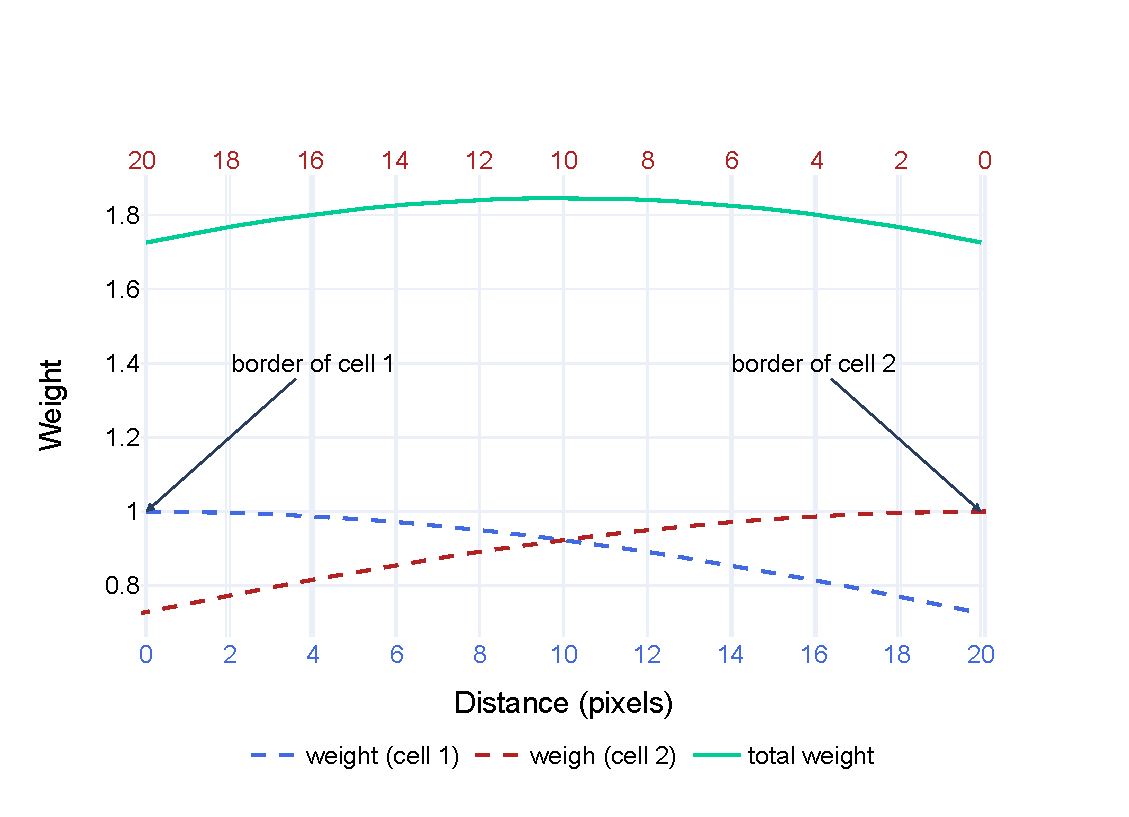
\includegraphics[width=\textwidth]{figures/130_methods/weight_calculation.eps}
%         \caption{Weight compounding}
%         \label{fig:weight_calculation}
%      \end{subfigure}
%      \begin{subfigure}[]{0.62\textwidth}
%          \centering
%          \includegraphics[ width=0.45\textwidth]{figures/130_methods/crop_mask_2451_crop.jpeg}
% \includegraphics[trim=0 0.008in 0 0, width=0.50\textwidth]{figures/130_methods/crop_weigths_2451_crop.jpeg}
%          \caption{Mask and correspondent weight map}
%          \label{fig:weight_map_example}
%      \end{subfigure}
% }
% \caption{\textbf{Weight map}. 
% \ref{fig:weight_calculation} shows the weight factors of background pixels between cells according to Eq. (\ref{weight_formula}). The dashed curves depict the weights generated by single cells as a function of the distance from their borders.
% % , respectively cell 1 on the left (blue) and cell 2 on the right (red).
% The green line illustrates the final weight obtained by adding individual contributions. 
% In \ref{fig:weight_map_example}, a target mask and the corresponding weight map.} 
% \label{fig:weight_map}
% \end{figure}
%
\begin{figure}
    \centering
    \includegraphics[width=\textwidth]{figures/130_methods/weights_calculation.pdf}
    \caption{\textbf{Weight compounding.}
    The dashed curves depict the weights generated by single cells as a function of the distance from their borders according to \cref{eq:weight_formula}.
    The green line illustrates the final weight obtained by adding individual contributions
    }
    \label{fig:weight_calculation}
\end{figure}
%
\begin{figure}
    \centering
    \subfloat[Mask]{
    \includegraphics[width=0.45\textwidth]{figures/130_methods/crop_mask_2451_crop.jpeg}
    }
    \subfloat[Weight map]{
    \includegraphics[trim=0 0.008in 0 0,
    width=0.50\textwidth]{figures/130_methods/crop_weights_2451_crop.jpeg}
    }
    \caption{\textbf{Weight map.} A target mask and the corresponding weight map}
    \label{fig:weight_map_example}
\end{figure}
%
The pseudocode\footnote{full implementation \githubweights} for a weight map is reported in Alg. \ref{algo:pseudocode_weightmap}, and an example weight map is shown in \cref{fig:weight_map_example}.

\begin{algorithm}%[H]
% \begin{algorithmic}[1]
\DontPrintSemicolon
     Initialize empty $\text{map}_j$ (mask size)\tcp*{weight map $j$-th mask}
    \For{each cell in mask} 
    {
    \tcc{loop over $i$-th cell in $j$-th mask}
         Initialize empty $\text{map}_i$  (mask size) \tcp*{weight map $i$-th cell}
        
         Add $i$-th cell to $\text{map}_i$
        
         Compute euclidean distance between each pixel of $\text{map}_i$ and the closest pixel of the $i$-th cell \label{step:distance}
        
         Compute each pixel's weight in $\text{map}_i$ according to a decreasing exponential function:
        \begin{equation}
        % \hskip 4.5cm
        \text{weight} = \exp\left\{\dfrac{-d^{2}}{2\sigma^{2}}\right\}
        \label{eq:weight_formula}
        \end{equation}
        
        \tcc {$d$ is the distance computed at step \ref{step:distance}}
        \tcc {$\sigma$ is a customizable parameter set to 25 (average cell radius)}
        
    Sum the resulting $\text{map}_i$ to the full $\text{map}_j$
    % , as illustrated in Fig. \ref{fig:weight_calculation};
}
% \end{algorithmic}
\caption{weight map pseudocode for $j$-th mask}
\label{algo:pseudocode_weightmap}
\end{algorithm}

% \section{Model training}
\label{sec:model_training}

After randomly setting 70 full-size images apart as a test set, the remaining pictures were randomly split into training and validation sets. 
In particular, twelve $512\times512$ partially overlapping crops were extracted from each image and fed as input to the network after undergoing a standard augmentation pipeline. Common transformations were considered as rotations, addition of Gaussian noise, brightness variation and elastic transformations \cite{elastic_tranformation}. 
The augmentation factors of the crops were fixed differentially based on their contents. 
The six patches included in the artifact oversampling ablation study were re-sampled 25 times each.
Instead, all the remaining crops produced 10 augmented versions for manually segmented images and 4 for all the others.
As a result, the model was trained on a total of nearly 16000 images (70\% for training and 30\% for validation).

All competing architectures were trained from scratch under the same conditions to favor a fair comparison.
Specifically, the Adam \cite{adam} optimizer was employed with an initial learning rate of 0.006. A scheduled decrease of 30\% was then applied if the validation loss did not improve for 4 consecutive epochs. 
A \textbf{weighted binary cross-entropy} loss was adopted on top of the weight maps to handle the imbalance of the two classes (weights equal to 1.5 and 1 for cells and background, respectively).
All models were trained until no improvement was observed for 20 consecutive epochs. In this way, each model was allowed to converge and the comparison was made at the best of each architecture's capabilities.

The approach was implemented through Keras API \cite{keras} using \texttt{TensorFlow} \cite{tensorflow} as backend. For more details, please refer to the GitHub repository\footnote{\github}.
The training was performed on 4 V100 GPUs provided by the \textit{Centro Nazionale Analisi Fotogrammi} (CNAF)\footnote{\cnaf} computing center of the \textit{National Institute for Nuclear Physics}\footnote{\infn} in Bologna.
In terms of 
% \section{Post-processing} \label{sec:post_processing}

% \begin{figure}
%     \begin{subfigure}{\textwidth}
%         \centering
%         \includegraphics[width=\textwidth]{figures/130_methods/orig+heatmap:278.png}
%         \caption{
%         % Original image and raw output
%         }
%         \label{fig:raw_output}
%         \end{subfigure}
%     \begin{subfigure}{\textwidth}
%         \centering
%         \includegraphics[width=\textwidth]{figures/130_methods/thresh+post_proc:278.png}
%         \caption{
%         % Thresholded and post-processed predicted masks
%         }
%         \label{fig:thresh+post_proc}
%         \end{subfigure}
%     \caption{\textbf{Model output}. 
%     Top: the input image with white contours indicating annotated cells  (left) and the model's raw output  (right).
%     Bottom: the predicted mask after thresholding at 0.875 (left) and the predicted mask after post-processing (right).}
%     \label{fig:model_output}
% \end{figure}
\begin{figure}
    \centering
    \subfloat[ground-truth]{
    \includegraphics[width=0.5\textwidth]{figures/140_results/orig:278.pdf}\label{fig:ground_truth}
    }
    \subfloat[raw heatmap]{
    \includegraphics[%trim=0 0.008in 0 0,
    width=0.54\textwidth]{figures/140_results/heatmap:278.pdf}\label{fig:heatmap}
    }
    
    \subfloat[thresholded prediction]{
    \includegraphics[width=0.5\textwidth]{figures/140_results/thresh:278.pdf}\label{fig:thresh}
    }
    \subfloat[post-processed prediction]{
    \includegraphics[width=0.5\textwidth]{figures/140_results/post_proc:278.pdf}\label{fig:post_proc}
    }
    \caption{\textbf{Model output}. 
    Top: the input image with white contours indicating annotated cells  (left) and the model's raw output  (right).
    Bottom: the predicted mask after thresholding at 0.875 (left) and the predicted mask after post-processing (right).}
    \label{fig:model_output}
\end{figure}
The final output of the model is a probability map (or heatmap), in which each pixel value represents the probability of belonging to a cell. 
% An example of this outcome is reported on the right of the \ref{fig:raw_output} if the input image on the left is provided to the model.
\Cref{fig:raw_output} reports an example of an input image (left) and the corresponding predicted heatmap (right).
% An example of this outcome is reported in the Fig. \ref{fig:raw_output} (right) if a sample input image (left) is provided to the model.
The higher the value, the higher is the confidence in classifying that pixel as signal. 
A thresholding operation was then applied on the heatmap to obtain a binary mask where groups of white connected pixels represent the detected cells. \Cref{fig:thresh+post_proc} (left) illustrates the cells detected after the binarization with different colors.
After that, ad-hoc post-processing was applied to remove isolated components of few pixels and fill the holes inside the detected cells. 
Finally, the watershed algorithm \cite{watershed} was employed with parameters set based on the average cell size.
\sidenote[Luca][notesyellow]{Descrivere meglio aggiungendo riferimenti nell'immagine}
An example of the results if provided in \cref{fig:thresh+post_proc}, where the overlapping cells in the middle present in the binary mask (left) are correctly splitted after post-processing (right). Also, the small object in the top right corner is removed
% , and the hole in the bottom right object is filled
.


\section{Model evaluation} \label{sec:model_evaluation}

% The Unet, small Unet, ResUnet and c-ResUnet architectures were evaluated and compared based on both detection and counting performance. 
All the presented approaches were evaluated and compared based on both detection and counting performance. 
Also, ablation studies were conducted to assess the impact of artifacts oversampling and weight maps.
% Also, ablation studies assessed the impact of artifacts oversampling and weight maps.

In order to evaluate the detection ability of the models, a dedicated algorithm was developed.
% Specifically, each target cell was compared to all objects in the corresponding predicted mask and uniquely associated with the closest one.
Specifically, each predicted object was compared to all cells in the corresponding ground-truth label and uniquely associated with the closest one.
If the distance between their centroids was less than a fixed threshold (50 pixels, i.e. average cell diameter), the predicted element was considered a match and it increased the true positive count (TP).
% ; a false negative otherwise (FN).
At the end of this procedure, all true objects without matches were considered as false negatives (FN). Likewise, the remaining detected items not associated with any target were considered as false positives (FP).
Algorithm \ref{algo:pseudocode_metrics} reports the pseudocode of the procedure described above\footnote{full implementation \githubmetrics}.
\begin{algorithm}%[H]
% \begin{algorithmic}[1]
    \DontPrintSemicolon
    % init
    \KwIn{ pred$_i$, mask$_i$}
    \KwOut {TP, FP, FN}       
    % \tcp*{true positives, false positives, false negatives}
    
    Set TP, FP, FN = 0
    
    Get predicted objects, pred\_objs$^i$
    \tcp*{detected cells}
    
    Get true objects, true\_objs$^i$
    \tcp*{annotated cells}
    
    % centers
    Get predicted centers, pred\_ctrs$^i$
    %  \tcp*{centers of predicted objects}
    
    Get true centers, true\_ctrs$^i$
    %  \tcp*{centers of true objects}
    
    \For{each ctr$_j$ in pred\_ctrs$^i$} 
        {
        \tcc{loop over predicted centers}
        \For{each ctr$_k$ in true\_ctrs$^i$}
            {
            \tcc{loop over true centers}
            
             Compute euclidean distance between ctr$_j$ and ctr$_k$ \label{step:ctrs_distance}
             
             Store distance and indexes
             \label{step:store_distance}
            } 
        
         Compute the minimum, min\_dist$_i$ of the distances stored in step \ref{step:store_distance}
         
        \If{understand}{
            Increase true positives, TP
            
            Remove ctr$_j$ from pred\_ctrs$^i$
            
            Remove ctr$_k$ from true\_ctrs$^i$
        }
        
        }
        
    Compute false negatives as true\_objs$^i$ - TP
    
    Compute false positives as pred\_objs$^i$ - TP
    
\caption{metrics computation for i\emph{-th} image}
\label{algo:pseudocode_metrics}
\end{algorithm}
Starting from these values, we referred to accuracy, precision, recall and $F_1$ score as indicators of detection performance.
% In terms of detection performance, the $F_1$ score was adopted as the primary indicator. Accuracy, precision and recall were also inspected to have a better understanding of the model ability. 
The definitions of such metrics are reported below:

\begin{align}
% \hskip 2cm
\text{accuracy} &=  \frac{\text{TP}}{\text{TP} + \text{FP} + \text{FN}}
= \frac{\text{1}}{\text{1} + \frac{1}{\text{TP}} \left(\text{FP} + \text{FN}\right)}
\label{eq:accuracy}; \\ 
\text{precision} &=    \frac{\text{TP}}{\text{TP} + \text{FP}}; \\
\text{recall} &=    \frac{\text{TP}}{\text{TP} + \text{FN}}; \\ 
F_1 \text{score} &=  \frac{2 * \text{precision} * \text{recall}}{\text{precision} + \text{recall}}
= \frac{2*\text{TP}}{2*\text{TP} + \text{FP} + \text{FN}} 
= \frac{\text{1}}{\text{1} + \frac{1}{\text{2TP}} \left(\text{FP} + \text{FN}\right)}
\label{eq:F1}.
\end{align}
% where TP, FP and FN indicates true positive (cells correctly detected), false positives (cells erroneously detected) and false negatives (cells erroneously missed), respectively. 
Notice that we do not have true negatives in \cref{eq:accuracy} since the prediction of the class ``not cell" is done at the pixel level and not at the object level, so there are no ``non-cell" objects predicted by the model.

Regarding the counting task, the Mean Absolute Error (MAE), Median Absolute Error (MedAE) and Mean Percentage Error (MPE) were used instead. More precisely, let $n_{\text{pred}}$ be the number of detected cells in $i$-th image  and $n_{\text{true}}$ be the actual one. Then, the absolute error (AE) and the percentage error (PE) were defined as:

\begin{align}
% \hskip 2cm
\text{AE} &= \lvert n_{\text{true}} - n_{\text{pred}}\rvert ;\\
\text{PE} &= \frac{ n_{\text{true}} - n_{\text{pred}}}{n_{\text{true}} 
% + \epsilon
}.
\end{align}
% where $\epsilon=10^{-6}$ was added to prevent a vanishing denominator when $n_{\text{true}} = 0$. 
Hence, the above counting metrics are just the mean and the median of the AE and the PE.
% The $F_1$ score was adopted for measuring the detection performance, while Mean Absolute Error (MAE), Median Absolute Error (MedAE) and Mean Percentage Error (MPE) were used as counting metrics. 

% \noindent\textbf{Threshold optimization}.
\subsection{Threshold optimization}

The choice of the optimal cutoff for binarization was based on the $F_1$ score computed on full-size images. In practice, DL models were evaluated on a grid of values and the best one was selected according to the \textit{Kneedle} method \cite{kneedle}. 
The same was done for the non-ML approach, with the only difference of considering the cutoff yielding the maximum $F_1$ value. 
The resultant thresholds were then used to assess performances on the test set.
Although the ultimate goal is retrieving the counts, we relied on detection performance to enforce accurate recognition and avoid spurious balancing between false positives and false negatives -- which are indistinguishable from the counts.
Also, full-size images (as opposed to crops) are used to simulate better the model performance in a real-world scenario.
\begin{figure}
\centerline{
\includegraphics[width=\textwidth]{figures/130_methods/F1_optimization.pdf}
}
\caption{\textbf{Threshold optimization}. On the left, the $F_{1}$ score computed on validation images as a function of the cutoff for thresholding.
On the right, the test $F_1$ score of the c-ResUnet model is used to illustrate the selection of the best threshold for binarization according to \textit{argmax} (blue) and \textit{kneedle} (red) methods.
} 
\label{fig:thresh_opt}
\end{figure}
% If the distance between their centroids was less than a fixed threshold (50 pixels, i.e. average cell diameter), the predicted element was considered a true positive; a false negative otherwise.
% Detected items not associated with any target were considered as false positives instead.

\Cref{fig:thresh_opt} shows the optimization results. On the left, we can see how each model performance varies in the validation set as a function of the cutoff for binarization.
For the adaptive thresholding approach, only very high thresholds lead to acceptable performances and we observe a sharp peak followed by a rapid decrease thereafter.
% Even though lower thresholds work best for all DL models, the $F_1$ curves are rather flat after their peaks. 
On the contrary, all DL models work best for lower thresholds and present $F_1$ curves which are rather flat after their peaks.
Thus, increasing the cutoff allows focusing only on predictions whereby the model is very confident, with just a slight loss in overall performance.
Also, good practices in natural science applications suggest being conservative with counts and only consider clearly stained cells.
For these reasons, we opted for the \textit{argmax} value (0.994) for the baseline approach, while we resorted to the \textit{Kneedle} method \cite{kneedle} for the selection of the optimal DL threshold. 
An example of that choice in the case of c-ResUnet is reported in \cref{fig:thresh_opt} (right).

% \chapter{Results}
\label{chap:partI_results}

After the training, the four competing architectures and the non-ML baseline are compared in three different scenarios: full design, weight maps only (no AO) and artifacts oversampling only (no WM). 
The 70 full-size images of the test set are used as a testbed.
\Cref{tab:metrics} reports individual model performances in terms of both detection and counting ability.
\begin{table}[H]
\centering
\resizebox{\textwidth}{!}{\begin{tabular}{lr|rrrrr|rrrr}
\toprule
Model &  Threshold &      $\boldsymbol{F_1 }$ & \textbf{AUC} & Accuracy &  Precision &  Recall & $\boldsymbol{R^2}$ &  \textbf{MAE} &  MedAE &     MPE (\%) \\
\midrule
\textbf{c-ResUnet}          &      \textbf{0.875} &  \underline{\textbf{0.8149}} & \underline{\textbf{0.8705}} &    \textbf{0.6877} &     0.9081 &  \textbf{0.7391} & \underline{\textbf{0.8215}} &  \underline{\textbf{3.0857}} &    \textbf{1.0} & -5.13 \\
c-ResUnet (no AO)  &      0.875 &  0.8047 & 0.8741 &    0.6732 &     0.9019 &  0.7264 & 0.8077 &  3.0857 &    1.5 & -6.24 \\
c-ResUnet (no WM)  &      0.875 &  0.7613 & 0.8594 &    0.6147 &     0.9418 &  0.6389 & 0.7048 &  3.6857 &    \textbf{1.0} & -19.14 \\
\midrule
ResUnet            &      0.850 &  0.7855 & 0.8579 &    0.6468 &     0.8865 &  0.7052 & 0.7831 &  3.3286 &    \textbf{1.0} & \textbf{-4.84}  \\
ResUnet (no WM)    &      0.850 &  0.7513 & 0.8643 &    0.6016 &     0.9387 &  0.6262 & 0.6955 &  4.0571 &    2.0 & -24.12 \\
Unet               &      0.875 &  0.7724 & 0.8609 &    0.6291 &     0.9117 &  0.6700 & 0.7560 &  3.5143 &    1.5 & -14.36 \\
Unet (no WM)       &      0.850 &  0.7886 & 0.8461 &    0.6510 &     0.8989 &  0.7024 & 0.8069 &  3.1571 &    2.0 & -9.23 \\
small Unet         &      0.875 &  0.7563 & 0.8691 &    0.6081 &     0.9264 &  0.6389 & 0.7682 &  3.5714 &    2.0 & -21.37 \\
small Unet (no WM) &      0.825 &  0.6697 & 0.8326 &    0.5034 &     \textbf{0.9483} &  0.5176 & 0.5723 &  4.7714 &    2.0 & -32.01 \\
\midrule
Adaptive Threshold &      0.994 & 0.6106 & 0.0865 &	0.4394 &	0.5680 &	0.6601  & 0.3565 &	8.0143 &	6.0 &	78.26 \\
\bottomrule
\end{tabular}}
\caption{\textbf{Performance metrics.}
Test set performance using the optimal \textit{kneed} threshold. The first five columns report the detection metrics, while the latter ones evaluate counting performance.
}
\label{tab:metrics}
% \end{center}
\end{table}

% \noindent\textbf{Performance}.
\section{Performance}

% By looking at the main figures of merit ($F_1$ score and MAE), it is clear how deep learning approaches perform better than the adaptive thresholding.
As a first observation, it is soon apparent how deep learning approaches perform better than adaptive thresholding according to all the considered metrics.

Starting with detection performance,
% as measured principally through the $F_1$ and AUC scores,
c-ResUnet clearly outperforms all competitors in terms of $F_1$ score.
% c-ResUnet clearly outperforms all competitors.
Remarkably, the Unet is consistently worse than c-ResUnet and ResUnet despite having far more parameters (nearly 14M against 1.7M and 887k, respectively).
The advantage of the ResUnet architectures is even more evident with respect to the lighter Unet version which has a comparable number of parameters (876k).
The values of the area under the precision/recall curves also confirm this supremacy. While the $F_1$ can be interpreted as a measure of maximum performance achieved, the AUC can be even more powerful since it indicates a global measure of performance independent of the choice of the threshold for binarization (see \cref{fig:results:PR}). Again, c-ResUnet sits on top of the list, with ResUnet and Unet following shortly after. Interestingly, the small Unet performs on par according to the AUC metrics, suggesting that the choice of the threshold is perhaps suboptimal for the test set.
\begin{figure}
    \centering
    \includegraphics[width=\textwidth]{figures/140_results/PR_test.pdf}
    \caption{\textbf{Precision/Recall plot.} 
    Test set precision/recall curves varying the threshold for predicted heatmap binarization. The inset plot reports a zoom of the top right corner to highlight differences of the various curves.}
    \label{fig:results:PR}
\end{figure}

In addition, c-ResUnet keeps its leading role also when extending the evaluation to the other metrics.
The only meaningful exception is precision, for which the Unet architectures are better. This is probably due to a tendency to overdetection. 
Nonetheless, the ResUnet counterparts well balance this behaviour with a significant improvement in accuracy and recall.

c-ResUnet remains the most accurate model also when shifting the focus on counting performance. Although the difference is hardly noticeable concerning the MAE, the gap becomes more prominent when looking at the $R^2$, with the \mbox{c-ResUnet} reaching a decent value of roughly 82\% of explained variability.
Interestingly, this time the ranking between ResUnet and Unet is inverted, with the latter performing slightly better in terms of counting.

Finally, it is worth noticing that adopting the kneed optimal threshold ensures large cutoffs and enforces only detections with high confidence.
Although desired, this behavior also increases false negatives as less cells are detected. 
As a result, we observe a drop in the accuracy whereby the impact of false negatives is twice as much the one in the $F_1$ score (cf. \cref{eq:accuracy,eq:F1}), thus explaining the gap between these two metrics.
% As a result, we observe a drop in the measures that are more impacted by false negatives, which explains the lower value of the accuracy compared to the $F_1$ score.
In conclusion, the model provides reliable predictions and satisfies the design requirement of being conservative with counts, as suggested by the negative values of MPE for all experimental conditions.

\begin{figure}[!b]
% \begin{wrapfigure}{R}{0.55\textwidth}
\centering
\includegraphics[width=\textwidth]{figures/130_methods/weigths_effect.png}
\caption{\textbf{Weight map effect.} 
Predicted heatmaps obtained with c-ResUnet (top row) and c-ResUnet (no WM).} 
\label{fig:weigths_effect}
% \end{wrapfigure}
\end{figure}
\section{Design evaluation}

This section presents the comparison of the different design choices investigated through the ablation studies.
In order to evaluate the impact of artifacts oversampling and weight maps, the experiments were repeated under the same conditions described in \cref{sec:model_training}, alternately switching off one of the two design choices.

From \cref{tab:metrics} it is evident how penalizing errors in crowded areas generally has a positive impact. Indeed, experiments exploiting weight maps achieve consistently better results than those without this addition (no WM). The only exceptions are the Unet and ResUnet architectures -- the former in terms of $F_1$ score, MAE and $R^2$, and the latter concerning AUC.  
In particular, this strategy seems to produce a loss in precision to foster a more significant gain in accuracy and recall.
\Cref{fig:weigths_effect} illustrates a visual comparison of the c-ResUnet output in crowded areas with (top) and without (bottom) weight maps. 
Again, its beneficial contribution is apparent, with close-by cells sharply separated when exploiting the weight maps.

Regarding the impact of artifacts augmentation, \cref{tab:metrics} shows how there is little difference between the full c-ResUnet and the one without oversampling of challenging examples (no AO).
In particular, the advantage of artifacts oversampling is numerically minimal.
This is also confirmed by qualitative evaluation (\cref{fig:predictions}).
On the one hand, the c-ResUnet (no AO) avoids detecting more evident biological artifacts as the stripe  in \cref{fig:predictions:noAO} even without specific oversampling.
On the other, the c-ResUnet  still fails to ignore the macaroni-shaped accumulation of fluorophore (\cref{fig:predictions:artifact}) although additional challenging examples are provided during training.
Probably, this is due to the lack of similar structures in the training set, which makes the oversampling ineffective for such kind of artifacts.
For this reason, the experiment was not replicated for the other architectures. 
% \begin{figure}
% \centerline{
%      \begin{subfigure}[]{0.55\textwidth}
%          \centering
% \includegraphics[width=\textwidth]{figures/140_results/pred_ResUnet_noAO:281.pdf}
%         \caption{
%         % c-ResUnet (no AO) prediction on artifact
%         }
%         \label{fig:predictions:noAO}
%      \end{subfigure}
%           \begin{subfigure}[]{0.55\textwidth}
%          \centering
% \includegraphics[width=\textwidth]{figures/140_results/pred_ResUnet:254.pdf}
%         \caption{
%         % c-ResUnet prediction on artifact
%         }
%         \label{fig:predictions:artifact}
%      \end{subfigure}
% }
% \centerline{
%           \begin{subfigure}[]{0.55\textwidth}
%          \centering
% \includegraphics[width=\textwidth]{figures/140_results/pred_ResUnet:168.pdf}
%         \caption{
%         % c-ResUnet prediction on artifact
%         }
%         \label{fig:predictions:false-positives}
%      \end{subfigure}
%       \begin{subfigure}[]{0.55\textwidth}
%          \centering
% \includegraphics[width=\textwidth]{figures/140_results/pred_ResUnet:278.pdf}
%         \caption{
%         % c-ResUnet prediction on artifact
%         }
%         \label{fig:predictions:false-negatives}
%      \end{subfigure}
% }
% \caption{\textbf{Results on test images}. 
% % Top row illustrates AO effect. 
% The c-ResUnet (no AO) correctly handles the evident stripe in the top left corner (\hyperref[fig:predictions:noAO]{a}), while the c-ResUnet fails with the macaron-shaped artifact (\hyperref[fig:predictions:artifact]{b}).
% % Bottom row highlights c-ResUnet predictive ability. 
% Also, notice how false positives (\hyperref[fig:predictions:false-positives]{c}, red boxes) look like target cells. Likewise, the objects discarded (\hyperref[fig:predictions:false-negatives]{d}, blue boxes) are similar to other stains that were not annotated.
% } 
% \label{fig:predictions}
% \end{figure}

% \savegeometry{origigeom}
% \clearpage
% \newgeometry{lmargin=1.5cm}
% \begin{landscape}
% \begin{figure}[!b]
%     \centering
%     \subfloat[\textit{Challenges:}
%     ]{
%     \includegraphics[width=\linewidth]{figures/140_results/pred_ResUnet:254.pdf}\label{fig:artifacts:clumping}
%     }
%     \caption{\textbf{Challenges and artifacts.}}
%     \label{fig:artifacts}
% \end{figure}%

% \begin{figure}[ht]\ContinuedFloat
%     \centering
%     \subfloat[\textit{Biological artifacts:} 
%     ]{
%     \includegraphics[width=\linewidth]{figures/120_dataset/challenges/stripe_and_filaments.pdf}\label{fig:artifacts:stripe}
%     }
%     \caption{\textbf{Challenges and artifacts. (2)}}
% \end{figure}%
% % \end{landscape}

% % \begin{landscape}
% \begin{figure}[ht]\ContinuedFloat
%     \centering
%     \subfloat[\textit{Technical artifacts:}
%     ]{\includegraphics[width=\linewidth]{figures/120_dataset/challenges/artifacts.pdf}\label{fig:artifacts:macaroon}
%     }
%     \caption{\textbf{Challenges and artifacts. (3)}}
% \end{figure}
% \end{landscape}
% \clearpage
% \restoregeometry


% \savegeometry{origigeom}
% \clearpage
% \newgeometry{lmargin=1.5cm}
% \begin{landscape}

% \begin{figure}[!b]
% \centering
% \subfloat[]{
% \includegraphics[width=\linewidth]{figures/140_results/pred_ResUnet_noAO:281.pdf}\label{fig:predictions:noAO}
% }
% \caption{\textbf{Results on test images}. 
% % Top row illustrates AO effect. 
% The c-ResUnet (no AO) correctly handles evident artifacts (\ref{fig:predictions:noAO}, top left corner), while the c-ResUnet fails with more problematic structures (\ref{fig:predictions:artifact}).
% % Bottom row highlights c-ResUnet predictive ability. 
% Notice how false positives (\ref{fig:predictions:false-positives}, red boxes) look like target cells. Likewise, the objects discarded (\ref{fig:predictions:false-negatives}, blue boxes) are similar to other stains that were not annotated.
% } 
% \label{fig:predictions}
% \end{figure}
% \begin{figure}[ht]\ContinuedFloat
% \centering

% \subfloat[]{
% \includegraphics[width=\linewidth]{figures/140_results/pred_ResUnet:254.pdf}\label{fig:predictions:noAO}
% }
% \caption{\textbf{Results on test images}. 
% % Top row illustrates AO effect. 
% The c-ResUnet (no AO) correctly handles evident artifacts (\ref{fig:predictions:noAO}, top left corner), while the c-ResUnet fails with more problematic structures (\ref{fig:predictions:artifact}).
% % Bottom row highlights c-ResUnet predictive ability. 
% Notice how false positives (\ref{fig:predictions:false-positives}, red boxes) look like target cells. Likewise, the objects discarded (\ref{fig:predictions:false-negatives}, blue boxes) are similar to other stains that were not annotated.
% } 
% \label{fig:predictions}
% \end{figure}


% \begin{figure}[ht]\ContinuedFloat
% \centering
% \subfloat[]{
% \includegraphics[width=\linewidth]{figures/140_results/pred_ResUnet:168.pdf}\label{fig:predictions:noAO}
% }
% \caption{\textbf{Results on test images}. 
% % Top row illustrates AO effect. 
% The c-ResUnet (no AO) correctly handles evident artifacts (\ref{fig:predictions:noAO}, top left corner), while the c-ResUnet fails with more problematic structures (\ref{fig:predictions:artifact}).
% % Bottom row highlights c-ResUnet predictive ability. 
% Notice how false positives (\ref{fig:predictions:false-positives}, red boxes) look like target cells. Likewise, the objects discarded (\ref{fig:predictions:false-negatives}, blue boxes) are similar to other stains that were not annotated.
% } 
% \label{fig:predictions}
% \end{figure}


% \begin{figure}[ht]\ContinuedFloat
% \centering
% \subfloat[]{
% \includegraphics[width=\linewidth]{figures/140_results/pred_ResUnet:278.pdf}\label{fig:predictions:noAO}
% }
% \caption{\textbf{Results on test images}. 
% % Top row illustrates AO effect. 
% The c-ResUnet (no AO) correctly handles evident artifacts (\ref{fig:predictions:noAO}, top left corner), while the c-ResUnet fails with more problematic structures (\ref{fig:predictions:artifact}).
% % Bottom row highlights c-ResUnet predictive ability. 
% Notice how false positives (\ref{fig:predictions:false-positives}, red boxes) look like target cells. Likewise, the objects discarded (\ref{fig:predictions:false-negatives}, blue boxes) are similar to other stains that were not annotated.
% } 
% \label{fig:predictions}
% \end{figure}

% \end{landscape}

% \clearpage
% \restoregeometry




\begin{figure}[!b]
\centering
\subfloat[stripes and filaments]{
\includegraphics[width=\textwidth]{figures/140_results/pred_ResUnet_noAO:281.pdf}\label{fig:predictions:noAO}
}
\caption{\textbf{Results on test images}. 
The c-ResUnet (no AO) correctly handles the evident stripe in the top left corner despite not receiving dedicated oversampling for such biological structures
% Filaments are also correctly interpreted
} 
\label{fig:predictions}
\end{figure}
\begin{figure}[ht]\ContinuedFloat
\centering

\subfloat[technical artifacts]{
\includegraphics[width=\textwidth]{figures/140_results/pred_ResUnet:254.pdf}\label{fig:predictions:artifact}
}
\caption{\textbf{Results on test images (2)}. 
The c-ResUnet fails with the \mbox{macaron-shaped} artifact in the middle of the picture, suggesting that the oversampling strategy is not effective in this case. However, notice that no other similar artifacts are present in the training set
} 
\end{figure}


\begin{figure}[ht]\ContinuedFloat
\centering
\subfloat[false positives]{
\includegraphics[width=\textwidth]{figures/140_results/pred_ResUnet:168.pdf}\label{fig:predictions:false-positives}
}
\caption{\textbf{Results on test images (3)}. 
The c-ResUnet sometimes produces false positives (red boxes), i.e. it labels as cell structures that are not annotated by the researcher.
However, the difference with marked cells is marginal (cf. also with \hyperref[fig:predictions:false-negatives]{d}), suggesting that these errors may lie within the limits of arbitrariness intrinsic to the task
} 
\end{figure}


\begin{figure}[ht]\ContinuedFloat
\centering
\subfloat[false negatives]{
\includegraphics[width=\textwidth]{figures/140_results/pred_ResUnet:278.pdf}\label{fig:predictions:false-negatives}
}
\caption{\textbf{Results on test images (4)}. 
% Top row illustrates AO effect. 
The c-ResUnet is generally conservative in predictions, thus generating false positives (blue boxes).
However, these are similar to other stains that were not annotated (cf. also with \hyperref[fig:predictions:false-positives]{c}), thus falling again within the limits of operator's interpretation
} 
\end{figure}









% \savegeometry{origigeom}
% \clearpage
% \newgeometry{lmargin=1.5cm}


% \begin{figure}[!b]
% \centering
% \subfloat[]{
% \includegraphics[width=\textwidth]{figures/140_results/pred_ResUnet_noAO:281.pdf}\label{fig:predictions:noAO}
% }
% \caption{\textbf{Results on test images}. 
% % Top row illustrates AO effect. 
% The c-ResUnet (no AO) correctly handles evident artifacts (\ref{fig:predictions:noAO}, top left corner), while the c-ResUnet fails with more problematic structures (\ref{fig:predictions:artifact}).
% % Bottom row highlights c-ResUnet predictive ability. 
% Notice how false positives (\ref{fig:predictions:false-positives}, red boxes) look like target cells. Likewise, the objects discarded (\ref{fig:predictions:false-negatives}, blue boxes) are similar to other stains that were not annotated.
% } 
% \label{fig:predictions}
% \end{figure}
% \begin{figure}[ht]\ContinuedFloat
% \centering

% \subfloat[]{
% \includegraphics[width=\textwidth]{figures/140_results/pred_ResUnet:254.pdf}\label{fig:predictions:noAO}
% }
% \caption{\textbf{Results on test images}. 
% % Top row illustrates AO effect. 
% The c-ResUnet (no AO) correctly handles evident artifacts (\ref{fig:predictions:noAO}, top left corner), while the c-ResUnet fails with more problematic structures (\ref{fig:predictions:artifact}).
% % Bottom row highlights c-ResUnet predictive ability. 
% Notice how false positives (\ref{fig:predictions:false-positives}, red boxes) look like target cells. Likewise, the objects discarded (\ref{fig:predictions:false-negatives}, blue boxes) are similar to other stains that were not annotated.
% } 
% \label{fig:predictions}
% \end{figure}


% \begin{figure}[ht]\ContinuedFloat
% \centering
% \subfloat[]{
% \includegraphics[width=\textwidth]{figures/140_results/pred_ResUnet:168.pdf}\label{fig:predictions:noAO}
% }
% \caption{\textbf{Results on test images}. 
% % Top row illustrates AO effect. 
% The c-ResUnet (no AO) correctly handles evident artifacts (\ref{fig:predictions:noAO}, top left corner), while the c-ResUnet fails with more problematic structures (\ref{fig:predictions:artifact}).
% % Bottom row highlights c-ResUnet predictive ability. 
% Notice how false positives (\ref{fig:predictions:false-positives}, red boxes) look like target cells. Likewise, the objects discarded (\ref{fig:predictions:false-negatives}, blue boxes) are similar to other stains that were not annotated.
% } 
% \label{fig:predictions}
% \end{figure}


% \begin{figure}[ht]\ContinuedFloat
% \centering
% \subfloat[]{
% \includegraphics[width=\textwidth]{figures/140_results/pred_ResUnet:278.pdf}\label{fig:predictions:noAO}
% }
% \caption{\textbf{Results on test images}. 
% % Top row illustrates AO effect. 
% The c-ResUnet (no AO) correctly handles evident artifacts (\ref{fig:predictions:noAO}, top left corner), while the c-ResUnet fails with more problematic structures (\ref{fig:predictions:artifact}).
% % Bottom row highlights c-ResUnet predictive ability. 
% Notice how false positives (\ref{fig:predictions:false-positives}, red boxes) look like target cells. Likewise, the objects discarded (\ref{fig:predictions:false-negatives}, blue boxes) are similar to other stains that were not annotated.
% } 
% \label{fig:predictions}
% \end{figure}

% \clearpage
% \restoregeometry
% \chapter{Conclusions}
\label{chap:partI_conclusions}
In \cref{partI}, we tackled the issue of automating counting cells in fluorescent microscopy images through the adoption of Deep Learning techniques.

From the comparison of four alternative CNN architectures, the cell ResUnet (c-ResUnet) emerges as the best model amongst the investigated competitors.
Remarkably, the careful additions with respect to the ResUnet \cite{deep_resunet} -- i.e. a learned colorspace transformation and a residual block with 5$\times$5 filters-- enable the model to perform better than the original Unet \cite{unet} despite having seven times fewer parameters.

Also, the two design choices considered in the ablation studies provide an additional boost in model performance. 
On one side, the adoption of a weight map that penalizes errors on cell boundaries and crowded areas is definitely helpful to promote accurate segmentation and dividing close-by objects. 
On the other, the effect of artifacts oversampling is less evident.
Nonetheless, the combined impact of the two components guarantees better results than any of the two considered separately.

In terms of overall performance, the results are satisfactory. 
Indeed, the model predicts very accurate counts (\mbox{MAE = 3.0857}) and satisfies the conservative counting requirement, as testified by the negative MPE (-5.13\%).
The detection performance is also very good (\mbox{$F_1$ score = 0.8149}), certifying that the precise counts come from accurate object detection rather than a balancing effect between false positives and false negatives.

Finally, qualitative assessment by domain experts corroborates further the previous statements. 
Indeed, by visually inspecting the predictions is possible to appreciate how even erroneous detections are somewhat arguable and lay within the subtle limits of subjective interpretability of borderline cases (see \cref{fig:predictions:false-positives,fig:predictions:false-negatives}).


In conclusion, the proposed approach proved to be a solid candidate for automating current operations in many use cases related to life science research.
Thus, this strategy may bring crucial advantages in terms of speeding up studies and reducing operator bias both within and between experiments.
For this reason, by releasing the c-ResUnet model\footnote{\linkmodel} and the annotated data\footnote{\dataset}, we hope to foster applications in microscopic fluorescence and similar fields, alongside innovative research in Deep Learning methods.

\part{Operational Intelligence for Distributed Data Management Monitoring}
\label{partII}

% \chapter{Contribution}

% You may also put some code snippet (which is NOT float by default), eg: \cref{lst:random-code}.

% \lstinputlisting[float,language=Java,label={lst:random-code}]{listings/HelloWorld.java}
% \label{lst:random-code}

% \cref{lst:metrics-code}.

% \lstinputlisting[float,language=python,label={lst:metrics-code}]{listings/metrics.py}
% \section{Fancy formulas here}

\input{opint/700_introduction}
    \input{opint/710_HEP}
    \section{The Worldwide LHC Computing Grid}
\label{wlcg}

The Worldwide LHC Computing Grid (WLCG) \cite{bird2011computing} is a global collaboration that links up more than 170 computing centers in 42 countries, serving an audience of more than 12000 physicists all around the world. 
As of 2022, WLCG constitutes the largest computing grid in the world and it is supported by many associated national and international grids, such as the European Grid Initiative and the Open Science Grid, as well as many other regional grids.
Founded in 2002 by CERN, the WLCG mission is to provide computing resources to store, distribute and analyze the data generated by the Large Hadron Collider.

Given the scale and complexity of the LHC data, this requires massive storage facilities, immense computing power, global networking, tailored software, adequate personpower and, of course, funding.
In order to achieve such challenging goals, WLCG leverages a distributed computing paradigm, where resources are shared among member states and made equally available to all the partners, regardless of their physical location.
% In brief, WLCG guarantees a seamless access to computing resources which include data storage capacity, processing power, sensors, and visualization tools, the resources that are capable to process over two million tasks daily, leveraging over one million computer cores and 1 exabyte of storage \cite{opint2022}.
\begin{figure}
    \centering
    \includegraphics[width=\textwidth]{figures/220_introduction/WLCG-Tiers-2021_v3.png}
    \caption{\textbf{WLCG structure.} The Worldwide Large Hadron Collider Grid has a tiered structure organized into three levels and comprising more than 170 computing centers spread across 42 countries.
    The image is borrowed from the \href{https://wlcg-public.web.cern.ch/sites/default/files/inline-images/WLCG-Tiers-2021_v3.png}{WLCG website}.
    } \label{fig:wlcg}
\end{figure}
\Cref{fig:wlcg} summarizes the WLCG infastructure composition. 
The Worldwide Large Hadron Collider Grid is structured in 4 levels, called \textit{tiers}, differing in terms of computing resources, storage capabilities and delivered services. 
% Proceeding from the bottom of this architecture, each layer sees an increased number
Its bottom layers comprise a few computing centers having great amounts of storage and processing resources, ultra-fast network connectivity (up to 100 GB/s), and they are devoted to general processing tasks.
The shallower layers, instead, group many smaller data centers devoted to more specialized activities.
In particular, the CERN data center is located at the bottom of this infrastructure, constituting the cornerstone of the whole architecture. 
It is located in Geneve (Switzerland) and it is endowed with more than 73000 processor cores, providing around 20\% of the total compute capacity of WLCG.
In terms of activity, the Tier-0 is responsible for i) the management of the raw data streams coming from the LHC experiments and their archiving for safe-keeping, ii) the reconstruction of physical entities like particles energy and velocity starting from the raw read-outs recorded by the electronic equipment, and iii) the distribution of raw and reconstructed data to the next tier layers.
Moving up the WLCG architecture, we find 13 large computer centres of the \textit{Tier-1s}.
These are directly linked to the Tier-0 and contribute to WLCG operations with sufficient storage capacity and round-the-clock support for the users. They are responsible for i) the safe-keeping of a proportional share of raw and reconstructed data, ii) large-scale reprocessing and safe-keeping of corresponding output, iii) access and distribution of data to the next infrastructure levels, and iv) safe-keeping of Monte Carlo simulated data.
One of these Tier-1 sites is located in Bologna\footnote{\cnaf} and it represents one of the biggest data centers in Italy. Its facilities count 40000 CPU cores, 40 PB of disk storage, 90 PB of tape storage, and the center is connected to the Italian (GARR) and European (GEANT) research network infrastructure with more than 200 Gbps \cite{cnaf2019annualrep, dell2019cnaf}.
The subsequent layer involves around 160 \textit{Tier-2} sites. These are data centers offered by universities and other scientific institutes, which are connected 
% to some of the Tier-1 sites 
through regional networks. 
They essentially act as analysis facilities to perform specialized tasks as the experiments production jobs and the Monte Carlo simulated data, which are then either stored locally or shared across the infrastructure.
% Despite having storage resources, the Tier-2s are not required to archive data, so the outputs produced there are typically sent back to Tier-1s when they are intended to be shared (as in the case of Monte Carlo data).
Finally, the last rung of the ladder is constituted by \textit{Tier-3s}. These sites enormously vary in scale,  ranging from local computing resources like university clusters or even individual pc to large national analysis facilities.
In fact, they do not formally belong to the WLCG but solely serve as entry points to its infrastructure for end-users analyses.

Alongside the hardware facilities, the WLCG supplies also advanced software solutions to provide researchers with seamless access to resources in a transparent way, without needing to worry about where the computing resources are coming from or where the data are physically stored.
This means that users can request access to data or resources from one of the many entry points into the system, and the grid infrastructure will then take care of spawning all the needed processes under the hood.
This may entail establishing the user identity and its access rights to the various sources, checking their credentials, and searching for available sites that can provide the requested resources.

    \input{opint/800_operational_intelligence}
    \input{opint/810_DDM}
    \section{FTS transfer failures} \label{sec:FTS_failures}


In practice, occasional faults may happen at various levels during data transfers, which may include a wide range of root causes, provoking failures during the shipment of the files.
These errors may vary from naive ones -- e.g. a mistyped command or the request of an unavailable file -- to more severe software and hardware defects.
For instance, the requesting endpoint or archiving server might be temporarily unreachable (connection shortage).
Likewise, the requested data may be corrupted (checksum error) due to storage hardware faults or unstable connection (network problem).
Also, there might be timeouts when the shipment takes more than the pre-configured waiting window -- e.g. when the desired data are bigger than usual and/or must be retrieved from tape, thus requiring more time.
In addition, errors of different nature may often arise due to the interactions between miscellaneous middleware layers.
All of these factors, and more, can generate significant service disruptions and infrastructure malfunctions that require prompt intervention.
For this reason, data transfer processes are continuously monitored by teams of shifters. When an issue is detected, the operators report it through the Global Grid User Support (GGUS) ticketing system \cite{antoni2008ggus}, and experts and site maintainers take care of their solution.
To give an idea of the volumes involved, the ATLAS collaboration alone experienced an average traffic of more than 2 PB per day in 2019 \cite{calafiura2020design_report}, corresponding to roughly 1.5-2 million files moved each day.
Nearly 10\% of these transfers failed producing about 100-200k errors on a daily basis. 
In total, transfer failures generated more than 4k incident reports filed in 2019\footnote{\ggus} for all the LHC experiments (1141 for ATLAS only).
Due to the complexity of the infrastructure and its layered composition, understanding the problem root causes and fixing them demands a great human effort -- more than 100 ATLAS members were involved in 2019, corresponding to roughly 50 FTEs (Full-Time Equivalent)~\cite{jarka2019ftes} -- and it may entail undesired disservices.
The average solving time may vary from a few hours or days -- e.g. in the case of issues that are easy to solve or have already been dealt with in the past -- to entire weeks -- e.g. for unknown problems or more troublesome malfunctions that imply important software or hardware interventions.
In practice, the median solving time for incidents reported by the ATLAS, CMS and LHCb collaborations in 2019 was around 17 days, with a 90\textit{-th} percentile of 44 days and a long right tail extending over 100 days (see \cref{fig:ggus_time}).
\begin{figure}
    \centering
    \includegraphics[width=\textwidth]{figures/220_introduction/GGUS_time.pdf}
    \caption{\textbf{Tickets solving time.} Boxplot of the distribution of the solving time for GGUS incidents reported in 2019 by ATLAS, CMS and LHCb collaborations.}
    \label{fig:ggus_time}
\end{figure}
When a transfer failure happens,
the FTS log files are parsed and the transfers more relevant features are extracted and re-organized in a structured format. 
In particular, this involves collecting the exit status of each of the subsystems responsible for the transfer and appending them to compose a global error message.
This information is then exposed to the on-duty shifters along with other characteristics -- e.g. source and destination endpoints, file size, exchange protocol and so on -- and visualizations -- e.g. time evolution plots or site transfer efficiency -- for more in-depth investigations.
% \lc{Here goes some reference to the orders of magnitude at stake, i.e.: 
% \begin{itemize}
%     \item n. tranfers/day (whole or per virtual organization) --> can retrieve from FTS
%     \item ticket/year or month or day (whole or per virtual organization) --> how to retrieve that? is there any official source?
% \end{itemize}
% }

% \lc{Describe current operations and possibly volumes: 
% \begin{itemize}
%     \item Current operations: efficiency matrix + drill down (description + falls)
%     \item average solving time $\rightarrow$ how to retrieve that? is there any official source?
%     \item n. people involved (both shifters and sites) $\rightarrow$ how to retrieve that? is there any official source?
% \end{itemize}
% }
%Current operations are based on a site-centric monitoring approach that involves mainly manual, post-mortem reporting. In this approach, trained operators look at Grafana dashboards that act as a high-level overview of the systems status and try to spot hints of incorrect or undesired behaviours.
Current operations are based on a \textit{site-centric} approach where trained personnel monitors the status of the various services almost 24/7 and tries to spot hints of incorrect or undesired behaviors. In particular, the operators look at Grafana dashboards to get a high-level overview of the system. A usual starting point is the so-called efficiency matrix (\cref{fig:efficiency_matrix}), where the percentage of successful transfers is reported. The granularity level is customizable and it may range from global transfers between national cloud infrastructures involving more computing centers to a finer tracking of particular site exchanges or even specific endpoint links. 
When the efficiency falls below an acceptable threshold, typically 60-70\%, on-duty shifters start to investigate the issue at a lower level by checking \emph{i)} where the error happened, \emph{ii)} how many errors are produced, \emph{iii)} what is the time pattern (temporary, extended or cyclical) and \emph{iv)} which error messages are generated. 
However, this procedure gives rise to many false alarms as it is usual to encounter problems that do not represent a real concern. For instance, this may happen when few transfers are attempted so even a low number of errors imply a high failure rate, or when there are after-effects of a transient issue that had already been fixed. 
Also, sometimes unnecessary drill-down activity is performed for actual issues that were already known, as in the case of ongoing tickets or site downtimes, for which reporting is not required.
As a result, many human resources are employed in repetitive tasks of little scientific interest that would enormously benefit from automation. 

In addition to that, the site-centric strategy described above has some drawbacks. Firstly, monitoring focuses on spotting where issues occur, while understanding the actual root causes is typically demanded to site experts in a subsequent investigation.
Secondly, problems generating few error messages are usually ignored. This is natural, and to some extent desirable, as having limited resources forces us to address bigger malfunctioning first. However, that could be a potential pitfall in cases where promptly fixing a minor issue may prevent the rising of a more significant and longer to solve defect.

All these problems could be tackled programmatically by standardizing the logging output of all the services. In this way, neat error messages would point directly to the source of the problem, thus allowing complete automation. 
However, the distributed nature of the infrastructure hampers such an approach.
In fact, the opportunistic gathering of computing resources that led to WLCG entails many local configurations that are not easy to address using only a static strategy.
Therefore, all these considerations expose the need for an intelligent support tool for speeding up infrastructure management to meet the productivity requirements for the near future.

\begin{landscape}
\begin{figure}
    \centering
    \includegraphics[height=\textwidth]{figures/220_introduction/grafana_efficiency_matrix_narrow1.png}
    \caption{\textbf{Transfer efficiency matrix (Grafana).} Transfer sources are shown as columns and destinations as rows. The drop-down menus at the top allow for custom filtering at the desired level of granularity.}
    \label{fig:efficiency_matrix}
\end{figure}
\end{landscape}
    \input{opint/821_related_works}
    \input{opint/830_contribution}

\chapter{Methods}

This section presents a detailed description of an approach for dealing with File Transfer Service failures. % \cref{sec:FTS_failures}.
The main goal is to analyze FTS failed transfers and identify error categories as suggestions of potential issues to investigate further by human experts.
In terms of desiderata, the objective is to develop a tool independent of experiment-specific configurations and workflows. Hence, we focus on errors produced by FTS rather than other services which are adopted only by some collaborations, e.g. Rucio for ATLAS.
Likewise, a minimal experts' effort is required. For this reason, we embrace an unsupervised learning approach to force the model to learn autonomously from data without needing a costly labeling phase of previous failures.
As a byproduct, this strategy also avoids incurring expectation bias from prior (perhaps suboptimal) operative categorizations, and it enables discovering new failure patterns.

The proposed approach \cite[Section 2.19]{opint2022} is inspired by the pipeline described in \citeA{lin2016log}. %although only part of it has been developed since no knowledge base is available for our use case.
In particular, we adopt a 3-step workflow consisting of \textit{i)} vectorization, \textit{ii)} clustering and \textit{iii)} description stages. 
The last step of the original pipeline, i.e. checking recurrence, is excluded since no knowledge base is available for FTS failures.
Also, our work is conceptually similar to the strategy described in \citeA{clusterlog2021}. However, some major differences are present in the pre-processing, clustering and description stages%
, and they are discussed in detail in \cref{sec:pipeline}.
% to mitigate the limitations discussed in \cref{sec:related_opint}.

In practice, our pipeline is developed inside the Operational Intelligence software framework\footnote{\githubpyspark}, and it is implemented trying to cope with the runtime restrictions for online processing despite not renouncing model performance.
To achieve that, the \textit{Spark} \cite{zaharia2010spark} processing framework is used through the \texttt{pyspark} language to leverage the advantages of distributed computations for large data. 
In particular, the whole pipeline is executed through the \textbf{SWAN service} \cite{piparo2018swan} that allows CERN users to run \texttt{Jupyter Notebooks} connected to Spark clusters on the WLCG infrastructure.
Also, a careful pipeline design is adopted to alternate online and offline elaborations.
Specifically, the learning phase of the vectorization stage is performed once on a big set of data (see \cref{sec:vectorization} for more details) and it is freezed and re-used as is -- possibly updating it once in a while.
The clustering stage, instead, is performed online every day so to always expose the latest results to the shifters on-duty (see %Sections
\cref{sec:clustering,sec:viz,ch:opint-results}
% \ref{sec:clustering}, \ref{sec:viz} and \ref{ch:opint-results} 
% \cref{sec:clustering,sec:viz} and \cref{ch:opint-results} 
for more details).

\section{FTS errors categorization} \label{sec:pipeline}

The pipeline illustrated in this work comprises an initial pre-processing step followed by the \textit{vectorization}, \textit{clustering} and \textit{description} stages.
Although conceptually similar to the workflow described in \citeA{clusterlog2021}, our approach considers some substantial modifications concerning mainly the pre-processing and the clustering stages.
Indeed, we apply minimal pre-processing to limit hard-coded feature engineering and let the vectorization stage figure out linguistic features of the error messages -- e.g. grammar, syntax, lexicon and semantic -- on its own.
The rationale behind this choice is that the resulting representation should be more expressive, thus better modeling the semantic of the messages and easing the successive clustering phase.

The next subsections provide a thorough description of each stage of our pipeline.


% Although the workflow in
% \citeA{clusterlog2021} accounts for all these phases and could be adapted for FTS errors as is, it also presents some relevant drawbacks.
% First, the pre-processing and vectorization stages reduce all the principal sources of variability, turning the whole approach into something close to unique strings grouping (assuming a smart and flexible definition of unique strings). 
% For example,  the raw error messages are transformed into structured templates where the same placeholder replaces all parametric parts.
% This choice drastically decreases the data variability. Also, it hampers the usage of parameter values for error discrimination, potentially masking faults due to specific components, e.g. one particular file is corrupted and needs restoration, or a determined site/service is not responding.
% Moreover, performing principal components decomposition on the word2vec embedding further reduces the expressive power of the learned representation.
% Although the previous strategies are crucial to comply with the runtime and computing requirements of particular use cases, they seem to contrast the current best practices for text processing. 
% In fact,  the recent applications in NLP literature suggest exploiting the increased computing power of modern architectures to train bigger models with minimal hard-coded feature engineering. 
% The idea behind that is to let the model figure out linguistic features -- e.g. grammar, syntax, lexicon and semantic -- and relations among tokens, thus endowing the resulting model with increased expressive power.
% As a result, the previous strategies likely hinder learning an optimal embedding, perhaps questioning the need for the word2vec language model for text vectorization in the first place.
% Another drawback is that no auxiliary information concerning the transfer processes is considered alongside the error message. This potentially prevents the system from spotting higher-level correlations with transfer features not contained in the error string.

% In order to mitigate these limitations, our approach considers some major modifications concerning mainly the pre-processing and the clustering stages.
% The next subsections provide a thorough description of each step of our workflow.% and describe the main differences with respect to the alternatives.

\begin{figure}
    \centering
    \includegraphics[width=.5\textwidth]{figures/410_method/pipeline.pdf}
    \caption{Caption}
    \label{fig:my_label}
\end{figure}

\input{opint/911_preprocessing}
\input{opint/912_vectorization}
\subsection{Clustering} \label{sec:clustering}

The next step of the pipeline is the clustering stage.
Cluster analysis examines the task of grouping a set of objects based on a given measure of distance or similarity.
This is a well-studied topic typically conducted to discover underlying structures in data during exploratory analysis or pattern recognition.

One of the most intuitive and widely adopted strategies to tackle this problem is the so-called \textit{k-means} algorithm \cite{lloyd1982kmeans}.
This technique is an iterative local search solution, and it refers to a particular formulation of the problem where the number of output groups, $k$, is supposedly known.
The algorithm evolves in four simple steps, starting from this prior information and after establishing a suitable distance measure to express the similarity between data points.
\Cref{fig:kmeans-pipeline} summarizes the k-means pipeline from raw data to the final clusters discovered applied to some toy data points.
In the initialization phase, $k$ arbitrary centers (also named \textit{centroids}) are chosen uniformly at random from the data points (\cref{fig:kmeans-pipeline:init}). 
In the next step, the data are split into clusters by mapping each data point to the nearest center (\cref{fig:kmeans-pipeline:updateClusters}). 
Once the groups are formed, the centroids are re-computed as the center of mass of all points assigned to the corresponding cluster (\cref{fig:kmeans-pipeline:updateCentroids}).
Finally, the last two steps are repeated until a convergence criterion is met (\cref{fig:kmeans-pipeline:result}).
% \Cref{fig:kmeans-pipeline} illustrates an animation of the first iteration and the final result of the algorithm described above applied to some toy data points.

% \begin{figure}
%     \centering
%     \subfloat[raw data]{
%     \includegraphics[width=0.5\textwidth]{figures/410_method/kmeans/kmeans_data.pdf}
%     }
%     \subfloat[initialization]{
%     \includegraphics[width=0.5\textwidth]{figures/410_method/kmeans/kmeans_centroid2.pdf}
%     }
    
%     \subfloat[update clusters]{
%     \includegraphics[width=0.5\textwidth]{figures/410_method/kmeans/kmeans_updateCluster.pdf}
%     }
%     \subfloat[update centroids]{
%     \includegraphics[width=0.5\textwidth]{figures/410_method/kmeans/kmeans_updateCentroids.pdf}
%     }
%     \caption{\textbf{K-Means clustering.} The algorithm performs an iterative search by alternately grouping observations around cluster centers of mass and updating such centroids.}
%     \label{fig:kmeans-pipeline1}
% \end{figure}

% \begin{figure}
%     \centering
%     \subfloat[raw data]{
%     \includegraphics[width=0.4\textwidth]{figures/410_method/kmeans/kmeans_data.pdf}
%     }
%     \subfloat[final result]{
%     \includegraphics[width=0.4\textwidth]{figures/410_method/kmeans/kmeans_finalResult.pdf}
%     }
    
%     \subfloat[initialization first centroid]{
%     \includegraphics[width=0.4\textwidth]{figures/410_method/kmeans/kmeans_centroid1.pdf}
%     }
%     \subfloat[initialization second centroid]{
%     \includegraphics[width=0.4\textwidth]{figures/410_method/kmeans/kmeans_centroid2.pdf}
%     }
    
%     \subfloat[update clusters]{
%     \includegraphics[width=0.4\textwidth]{figures/410_method/kmeans/kmeans_updateCluster.pdf}
%     }
%     \subfloat[update centroids]{
%     \includegraphics[width=0.4\textwidth]{figures/410_method/kmeans/kmeans_updateCentroids.pdf}
%     }
%     \caption{\textbf{K-Means clustering.} The algorithm performs an iterative search by alternately grouping observations around cluster centers and updating centroids.}
%     \label{fig:kmeans-pipeline1}
% \end{figure}

\begin{figure}
    \centering
    % \subfloat[raw data]{
    % \includegraphics[width=0.5\textwidth]{figures/410_method/kmeans/kmeans_data.pdf}
    % }
    \subfloat[initialization]{
    \includegraphics[width=0.5\textwidth]{figures/410_method/kmeans/kmeans_centroid2.pdf}\label{fig:kmeans-pipeline:init}
    }
    \subfloat[update clusters]{
    \includegraphics[width=0.5\textwidth]{figures/410_method/kmeans/kmeans_updateCluster.pdf}\label{fig:kmeans-pipeline:updateClusters}
    }
    
    \subfloat[update centroids]{
    \includegraphics[width=0.5\textwidth]{figures/410_method/kmeans/kmeans_updateCentroids.pdf}\label{fig:kmeans-pipeline:updateCentroids}
    }
    \subfloat[final result]{
    \includegraphics[width=0.5\textwidth]{figures/410_method/kmeans/kmeans_finalResult.pdf}\label{fig:kmeans-pipeline:result}
    }
    \caption{\textbf{K-Means clustering.} The algorithm performs an iterative search by alternately grouping observations around the current centroids (\hyperref[fig:kmeans-pipeline:updateClusters]{b}) and updating the centers of the clusters (\hyperref[fig:kmeans-pipeline:updateCentroids]{c})}
    \label{fig:kmeans-pipeline}
\end{figure}

% \begin{figure}
%     \centering
%     \animategraphics[width=\textwidth, %loop,
%     autoplay]{1}{./figures/410_method/kmeans/gif/kmeans_}{0}{6}
%      \caption{\textbf{K-Means clustering.} The algorithm performs an iterative search by alternately grouping observations around cluster centers of mass and updating such centroids.}
%     \label{fig:kmeans-pipeline}
% \end{figure}

    
% \begin{figure}
%     \centering
%     \includegraphics[width=\textwidth]{figures/410_method/kmeans/K-Means++ diagram.pdf}
%     \caption{\textbf{K-Means clustering.} The algorithm performs an iterative search by alternately grouping observations around cluster centers of mass and updating such centroids.}
%     \label{fig:kmeans-pipeline}
% \end{figure}

In this study, we resort to clustering for grouping messages including similar content.
The resulting clusters are therefore interpreted as error categories.
In particular, we adopt a slight variation of the above algorithm referred to as \mbox{\textbf{k-means++}} \cite{arthur2006kmeans++}.
The two techniques share the same workflow except for how the starting centroids are initialized.  
Specifically, the \mbox{k-means} algorithm assigns equal probability to all the data points and then samples $k$ centers.
For \mbox{k-means++} instead, only the first centroid is chosen uniformly at random. The following $k-1$ centers are sampled from data points with probability inversely proportional to the distance between each point and the closest predefined centroid.
This careful seeding strategy ensures the initial centers are more spread across the data points, thus favoring better clustering results and a faster convergence.
Despite more advanced clustering algorithms are available and may be applied to our use case, e.g. DBSCAN \cite{ester1996dbscan}, HDBSCAN \cite{mcinnes2017hdbscan}, BIRCH \cite{zhang1996birch}, OPTICS \cite{ankerst1999optics}, spectral clustering \cite{ng2002spectral} and so on, the choice of the a \mbox{k-means} algorithm is justified by its intuitive approach and good performance in practice in a wide range of applications \cite{von2012clustering}.
Also, a perhaps more profound and substantial motive is that the clustering strategy may be seen as a functional but not primary pipeline stage. Indeed, the learned language model determines the geometry of the embedded space, thus influencing the point cloud shapes of different error categories. 
For this reason, we embrace the idea that a simple clustering algorithm is preferable, and particular attention must be devoted to tuning the vectorization stage for easing the subsequent clustering, possibly even fostering the learning of an optimal representation for a specific clustering algorithm \cite{yang2017kmeans-friendly}.

In order to demonstrate the approach, we report the analysis of FTS data from one full day of operation (2021-01-15), corresponding to roughly 1 M errors and 1.5 GB of data.
To help the successive evaluation phase, only transfers between Tier-0, Tier-1s and Tier-2s are considered in the analysis.
In practice, more hyper-parameter configurations are explored to test the effect of different choices.
The first set of investigations regards the measure of similarity adopted to form the clusters. 
In this respect, we tested two alternatives, cosine similarity and the euclidean distance.
The former consistently outperformed euclidean distance in all attempted experiments, 
both in terms of cluster geometrical properties and interpretability of the results.
% both considering clusters compactness and separation and in terms of interpretability of the results. 
For this reason, only the the analysis involving \textbf{cosine similarity} is reported in the following.

Another crucial hyper-parameter is given by the assumed number of clusters, $k$. This represents the number of error categories in our case, which is not known in advance. 
Therefore a grid search for $k \in [12, 15, 20, 30] $ is exploited to retrieve a reasonable estimate from the data.
For this purpose, two geometrical criteria are considered to compare results of different settings, namely the \textit{Within cluster Sum of Squared Errors} (WSSE) and the \textit{Average Silhouette Width} (ASW) \cite{rousseeuw1987ASW}.
The WSSE measures the internal cluster variability, so the lower its value, the better the performance.
In terms of its definition, the WSSE is based on the total sum of squared distances between the points of each group and the correspondent centroid:
\begin{equation}
    \text{WSSE}\left(\text{dist}, k\right) = 
    \sum_{j=1}^{k}{ 
    \sum_{x_i \in C_j}{\text{dist}\left( x_i - \bar{x}_j\right)} 
    }
\end{equation}
where $x_i$ is a generic data point, ${dist}$ is a desired distance measure, and $C_j$ and $\bar{x}_j$ indicate a generic cluster and its centroid, respectively.
Although compactness is certainly a desirable property for the output groups, this metric is strongly affected by the scale of the variables and the number of observations. Indeed, the clusters exhibit a greater variability as their points present higher values and/or the cluster size increases, thus causing the WSSE to explode. 
Also, being unbounded by its nature, i.e. $\text{WSSE} \in \left[ 0, +\inf \right]$, the WSSE is of difficult interpretation on its own and it only makes sense when compared to other values. \\
% In fact, its absolute value have little sense on its own, and it only takes meaning when compared to other.
A better metric is the so-called average silhouette width. In brief, the ASW is a measure of clustering performance that accounts for both internal homogeneity and external separation of the clusters.
In particular, let $\bar{a}_i$ be the average distance of $x_i$ from all the other points belonging to the same cluster $C_I$. Also, let $b_i$ be the minimum average distance of $x_i$ from the observations in all the other clusters $C_j , \forall j \neq I$. Then, the ASW is defined as:
\begin{equation}
    \text{ASW}\left(\text{dist}, k\right) = 
    \dfrac{1}{n} \sum_{i=1}^{n}{ 
    \dfrac{b_i - \bar{a}_i}{ \max\left( \bar{a}_i, b_i \right) }
    }
\end{equation}
where $n$ is the total number of observations, i.e. error messages in our case.
The average silhouette is much more intuitive to interpret than the WSSE as its value is bounded in the interval $\left[ -1, +1 \right]$.
In practice, negative values of the ASW mean that points of one cluster are on average more similar to observations of other groups than the ones of their own cluster. A value of 0, instead, suggest that the groups are not really distinguishable, thus making the assignation of single observations to any of the clusters arbitrary.
Finally, positive values close to 1 testify that the clustering produces nicely homogeneous groups that are also well separated.
Given the more intuitive reading of ASW values, the latter is used in the following as the main figure of merit.

% Apart from the distance and the value of $k$, the other hyper-parameters were not optimized and the values \textbox{initSteps=200}, \textbox{tol=0.0001}, \textbox{maxIter=100} were chosen.

The results of the comparison between WSSE and ASW for different values of $k$ are reported in \cref{fig:k_optim}.
Both indicators tend to improve as the number of clusters increases.
In particular, a value of $k=30$ clusters seems to be optimal according to both criteria.
Notably, however, the ASW indicator reaches very high values (around 0.9) even for lower $k$ values.
% of 0.9405 which is a very high score for this metric.
For this reason, the configuration having $\boldsymbol{k=15}$ is preferred to limit the number of suggested issues and minimize the shifters effort.
% considered for the discussion in \cref{ch:opint-results}. 

\begin{figure}
    \centering
    \includegraphics[width=\textwidth]{figures/410_method/kmeans/k_optim.pdf}
    \caption{\textbf{Optimization of $\boldsymbol{k}$.} The plot shows the value of the WSSE and ASW metrics as a function of the number of clusters, $k$. The hexagonal markers indicate the optimal values, which correspond to $k=30$ for both indicators}
    \label{fig:k_optim}
\end{figure}

\input{opint/914_description}

\input{opint/1000_results}
\input{opint/1010_interpretation}
\section{Quantitative assessment: GGUS tickets}
\label{sec:opint:quantitative}


The drawback of unsupervised techniques lies in the inherent difficulty of the evaluation phase, as no ground truth is available for comparison \cite{von2012clustering}.
In order to overcome this limitation,
% % and to avoid demanding the whole performance assessment to manual inspection and interpretation of the clustering results, we resort to the comparison 
% we have conducted extensive testing as pre-validation comparing the clusters obtained with our approach against GGUS tickets.
% In order to overcome the difficulty in measuring the goodness of the produced clusters, 
we have conducted extensive testing using incidents reported in GGUS as a benchmark. 
In this way, we attempt to provide a quantitative assessment of the pipeline performances and a more direct measure of its potential impact when applied in practice.
In particular, we explore the overlapping between discovered clusters and the reported issues in two directions expressing alternative perspectives to the problem. 
On one side, we evaluate the usefulness of our approach for the shifters, i.e. how clusters explain failures/tickets (\textit{direct association}).
On the other, we study the overall capacity of the pipeline to discover and highlight issues -- i.e. how many failures/tickets are reflected in the clusters (\textit{inverse association}).
In the first case, the objective is to limit the effort of the operators by suggesting as few potential failures as possible, meanwhile still highlighting the major concerns for the infrastructure. Thus, the focus is on limiting false positives at the expense of neglecting minor issues.
On the contrary, the second point of view requires a more comprehensive search aimed at isolating all the ongoing malfunctions, irrespectively of their current priority. Hence, this time the focus is on maximizing true positives.
\Cref{tab:cross-check} reports a summary of the evaluation according to both perspectives..
\newcommand{\specialcell}[2][c]{\begin{tabular}[#1]{@{}c@{}}#2\end{tabular}}
\begin{table}%[htb]
\centering
\resizebox{\textwidth}{!}{
\begin{tabular}{cccccccc}
\toprule
\textbf{N. Clusters} &  \textbf{ASW} &  \textbf{WSSE} &  \textbf{\specialcell{Perfect\\Match}} &  \textbf{\specialcell{Fuzzy\\Match}} &  \textbf{\specialcell{Partial\\Match}} & \textbf{\specialcell{False \\ Positives}} & \textbf{\specialcell{False \\Negatives}} \\
\toprule
     &       &        &     &    &    &    &   \\[-0.25cm]
  15 &  0.89 &  17107 &   7 &  3 &  2 &  3 &  1 \\[0.2cm]
\bottomrule  
\end{tabular}
}
\caption{Summary of pre-validation results.}
\label{tab:cross-check}
\end{table}

Concerning the first angle, we consider GGUS issues reported in a skewed time window of 17 days (01-01 to 01-18) around the day of the analysis for a total of 20 tickets related to data transfer failures.
Adopting this filtering strategy is convenient since it considers both previously known issues and delayed detections.
The former is necessary because standard practice in current operations requests not to open new incident reports when related investigations are already ongoing. Hence, considering only tickets opened on the analysis day may lead to incorrect conclusions.
Instead, the latter is convenient to account for a ``grace period" if the operators do not promptly spot failures that are really happening during the analysis.
Overall, a good level of agreement is observed between the 15 discovered clusters and the 20 tickets.
Specifically, the 7 \textit{perfect matches} indicate cases whereby the reported message and the affected site coincide with the ones highlighted by the clusters.
The 3 \textit{fuzzy matches}, instead, refer to occasions whereby the agreement is less obvious, meaning that the cluster has evident connections with more than one ticket.
Similarly, the 2 \textit{partial matches} describe cases whereby either the message or the site coincide. 
The previous three statistics reveal that 12 out of the 15 suggested failures have led to fruitful investigations, thus implying a precision between 0.46 and 0.8 depending on the degree of nuisance one is willing to tolerate. 
Besides the above matches, 3 clusters highlight issues not reported on GGUS in the considered time window.
These false positives indeed entail a futile effort for the operators and should be avoided, e.g. thwarting in-depth investigations 
if the temporal pattern is not escalating and/or the number of errors is not a concern.
Nevertheless, in our case, posterior checks on the 3 false positives showed hints for real problems that went undetected or unreported by the operators, i.e. the error pattern seemed similar to other incidents opened to different sites.

For the second assessment, we investigate the relationship between clusters and tickets in the opposite direction, i.e. by looking at how many reported issues our approach captures.
In this case, we consider a different baseline that provides a fairer detection performance evaluation.
Indeed, it is reasonable to think that the failures observed during the analysis may be correlated to earlier tickets, thus justifying the adoption of a wide time window for the direct association.
%the wide time window adopted earlier is justified by the possibility of observing new failures during the analysis which are correlated to past tickets.
 %not reported because related to open tickets.
%of open tickets for which new failures are observed during the analysis but not reported.
However, the same rationale does not necessarily apply when we reverse our perspective. In fact, there is no prior guarantee that a past ticket will generate new failures at a given moment in the future.
Hence, considering all tickets undergoing investigations would potentially bias our measurement since specific past failures may not produce new malfunctions during the day of the analysis, thus resulting in untruthful false negatives.
For this reason, in the case of the inverse association we limit our baseline to consider solely the tickets for which failures were really observed during the day of the analysis, thus reducing the initial 20 reports to only 9.
Given this reference framework, the clusters successfully identify 8 out of 9 tickets, thus overlooking only a single issue. 

To summarize, the previous results show that the approach presents promising perspectives given the complexity of the task and the completely unsupervised approach embraced.
Although conducting an indisputable quantitative assessment is challenging -- if not impossible with the available data --, the considerations expressed above furnish a reasonable proxy of the potential of our approach.
Of course, a trade-off between the two perspectives is desirable in practice, for which more tuning is necessary with the help of shifters and site experts. 

\chapter{Conclusions} \label{ch:opint:conclusion}

The increasingly growing scale of modern computing infrastructures solicits more ingenious and automatic solutions to their management.
This is particularly true concerning WLCG and the LHC experiments, whereby the upcoming upgrade will deliver ten times the actual volumes at a flat budget for infrastructure management.

\cref{partII} of this thesis discuss a data-driven pipeline to support DDM operations management for LHC experiments, with a particular focus on FTS transfer failures.
The proposed approach consists of a pipeline that takes care of all the steps of a typical data science project, from the raw data to the final visualization.
Also, some pre-production integration and testing has been made.
In particular, the approach is already compatible -- at least to some extent -- with the production systems as it natively interacts with the raw data streams, and it complies with the timely execution requirements for online processing.
In fact,
% the application of pre-trained vectorization and online clustering -- is compatible with online usage. 
the pipeline takes around 2.5/3 hours for one day of data, which is compatible with one or two applications per 8-hours shifts.
% Specifically, 
This runtime is almost equally divided among the clustering stage -- with a grid search for the optimization of $k$ as described in \cref{sec:clustering} -- and the post-processing/pre-aggregation needed for the visualization.
Furthermore, no specific effort to optimize such runtimes was attempted, which suggests that some space for improvement is probably still available.

In terms of performance, our pipeline delivers promising results. 
The output clusters show an evident ability to capture both structural and semantic similarity between messages, as discussed in \cref{sec:opint:qualitative}.
Remarkably, this result is achieved despite applying minimal hard-coded feature engineering and exploiting simple baseline models for vectorization and clustering. 

% Hence, the language model produced by (\textit{word2vec}) seems expressive enough to properly represent the error messages, perhaps due to their lower variability compared to natural language. 
% On top of that, the (\textit{k-means}) clustering performs reasonably well in separating error categories in the resulting embedded space.
% This outcome is somewhat surprising given the simplicity of the approaches, expecially regarding the k-means.

% Thus, rather than exploring more sophisticated alternatives for such methods, a possible direction for future extensions could be the adoption of techniques

% This outcome is somewhat surprising, especially regarding the k-means. In fact, 
Interestingly, incorporating additional auxiliary information related to the source and destination hostnames seems to help unravel higher-level interactions between the nature of the issues and where they occur.
This, in turn, provides a finer detail when spotting problems that may aid the human operators to restore the proper functioning of the infrastructure faster.

The previous considerations are also corroborated by a quantitative assessment of the pipeline's potential impact when applied to daily workflows. This is done by comparing the outputs of our approach to the incidents reported in GGUS in a reasonable time window around the day of the analysis.
In terms of the direct association between clusters and tickets, the performance varies from average to decent depending on how much nuisance one is willing to tolerate in the output.
Regarding the inverse relationship, instead, the approach is close to perfection since it highlights 8 out of the 9 incidents observable on the day of the analysis. 

Nonetheless, some adjustment and tuning would be helpful prior to full integration into production.
First, the analyzed clusters show indications that additional tuning may be needed in some cases to guarantee a more suitable level of granularity.
This task is highly application-specific and requires the direct involvement of shifters and site experts.

A second concern is related to the limited number of errors shown.
Ideally, the perfect output for our use case would be one error pattern
-- or even a more human-readable description directly pointing to the source of the problem -- 
per cluster for a small number of clusters (e.g. $\leq6$).
In practice, however, the magnitude of the problem still refers to the actual number of failures. Even reducing it to the minimum, this is still bounded by the number of combinations between unique strings/patterns and source/destination locations, which is clearly overwhelming to handle for human operators.
Therefore, the desired output is hardly deliverable as there is a trade-off between the clusters' internal homogeneity (number of patterns) and their number.
For this reason, we reach a compromise by setting a higher value of $k$ and displaying just a fixed portion of each cluster (3 patterns in the current implementation).
However, limiting the visualized patterns potentially hinders serious faults of medium and small sizes.
Moreover, the necessity to mask message parameters to get more informative and abstract descriptions prevents using their values for troubleshooting -- e.g. when the failures are due to specific parameter values.
In order to comply with the above requirements, a possible solution is a flexible and efficient implementation that allows the shifters to adjust the number of displayed patterns and enables interactive drill-down to investigate more closely the effect of parametric values.
Nevertheless, guaranteeing a good balance constitutes an intrinsic challenge of our use case, and its resolution again requires a direct tuning by experts.

Furthermore, although it makes sense to cross-check clustering results with GGUS tickets for a quantitative evaluation, this comparison has drawbacks. 
On one side, GGUS incidents force to focus solely on reported failures, thus preventing the study of undetected issues and masking some omission policies due to external factors -- e.g. the site is in downtime or blacklisted, or the fault is known to be transient and therefore not reported.
% it just needs some time for automatic recovery.
On the other side, the procedure is sensitive to the choice of the time window.
Indeed the issues may have no match because they are reported before the selected period or due to delays in their discovery and reporting. 
All in all, the final assessment may result biased because of these factors, thus limiting the reaches of the drawn conclusions.

All of the previous adjustments demand additional in-depth studies, each requiring a lengthy manual review of the results due to the unsupervised approach.
Also, most of the above solicit direct participation of system experts to guarantee the soundness of the results and proper tuning.
% a manual check of the ticket information and the cluster content, making the comparison lengthy and not scalable. 
Considering the several appointed investigations and the conspicuous number of alternative combinations, it becomes clear how the requested effort is not affordable and does not scale to the comparison of adversarial approaches.
A possible solution we envision for future developments is represented by the collection of a reference dataset where to store labels for error categories, root causes, incident priority and solving actions. 
In this way, the evaluation of new experiments would become immediate and systematic.
Also, this would make the investigation of novel techniques sustainable, enlarging the plethora of applicable approaches to supervised methods and enabling a coherent comparison of alternative algorithms.
Perhaps more importantly, the derived measure of performance would be linked to the actual goal of the analysis, thus allowing a direct optimization of the models for the specific task of interest.
%In this way, we will have a task-related measure of performance while easing the comparison of alternative algorithms and making the investigation of novel techniques sustainable.
%Pushing the target even further, enhancing the level of detail of the collected information would allow framing the problem in terms of more advanced tasks as Question Answering (QA) or Named Entity Recognition (NER). As a result, it would be possible to exploit tools available in the NLP literature to address the key problem related to transfer failures, i.e., understanding the root causes and suggesting solving actions for the issues.




% Finally, a problem is the fact that only a limited number of errors are shown.
% Although this number is customizable -- in our case is limited to 3 to avoid the confusions -- so a bigger number may be displayed if desired, this is an intrinsic challenge of our use case.
% In practice, the magnitude of the problem still refers to the actual number of failures. Even reducing it to the minimum, this is still bounded by the number of combinations between unique strings/patterns and source/destination locations, which is of course too big to handle for human operators.


% Although it makes sense to cross-check clustering results with the tickets, this comparison has drawbacks. 
% In particular, the procedure is sensitive to the choice of the time window.
% As a matter of fact, some issues may have no match because either reported before the time window starts or due to delays in their discovery and reporting. 
% Another limitation is that this comparison requires a manual check of the ticket information and the cluster content, making the comparison lengthy and not scalable.
% A possible solution is represented by the collection of a reference dataset where to store labels for error categories, root causes, incident priority and solving actions. 
% In this way, the comparison of alternative algorithms would become immediate and coherent, thus making the investigation of novel techniques sustainable.
% Perhaps more importantly, the derived measure of performance would be linked to the actual goal of the analysis, thus enabling a direct optimization of the models for the specific task of interest.
% %In this way, we will have a task-related measure of performance while easing the comparison of alternative algorithms and making the investigation of novel techniques sustainable.
% Pushing the target even further, enhancing the level of detail of the collected information would allow framing the problem in terms of more advanced tasks as Question Answering (QA) or Named Entity Recognition (NER). 
% As a result, it would be possible to exploit tools available in the NLP literature to address the key problem related to transfer failures, i.e., understanding the root causes and suggesting solving actions for the issues.

%----------------------------------------------------------------------------------------
% BIBLIOGRAPHY
%----------------------------------------------------------------------------------------

\backmatter

\part*{}

% \nocite{*} % comment this to only show the referenced entries from the .bib file

\bibliography{bibliography/c_resunet, bibliography/data_science, bibliography/part_II}
% \bibliography{bibliography/010_introduction}
\end{document}